\documentclass[conference]{IEEEtran}
\IEEEoverridecommandlockouts
% The preceding line is only needed to identify funding in the first footnote. If that is unneeded, please comment it out.
\usepackage{cite}
\usepackage{amsmath,amssymb,amsfonts}
\usepackage{algorithmic}
\usepackage{graphicx}
\usepackage{listings}
\lstset{breaklines=true}
\usepackage{url}
\usepackage{hyperref}
\usepackage{dirtree}
\graphicspath{ {images/} }
\usepackage{textcomp}
\usepackage{xcolor}
\usepackage{todonotes}
\usepackage{subcaption}
\usepackage{placeins}
\usepackage{comment}
\usetikzlibrary{positioning}
\usepackage{float}
\usepackage{tikz}
\usepackage{hyperref}
\usepackage{indentfirst}
\usetikzlibrary{calc, patterns, patterns.meta, shapes.geometric, arrows.meta, positioning, fit, decorations.pathreplacing, trees, arrows, shapes.misc, angles, quotes}
%Go-kart command \gokart{"x"}{"y"}{"rot_in_deg"}
\def\gokart#1#2#3{
    \begin{scope}[shift={(#1,#2)}, rotate=#3]
        \begin{scope}[shift={(0,-0.85)}] %Offset so (x,y) is the front bumper
            %Front bumper
            \draw[very thick] (-0.7, 0.75) -- (-0.5, 0.85) -- (0.5, 0.85) -- (0.7, 0.75);
            %Body
            \draw[fill=gray!30] (-0.5,-0.75) rectangle (0.5,0.75);
            %Wheels
            \draw[fill=black, rounded corners=0.75] (-0.6,0.6) rectangle (-0.4, 0.3); % Front left
            \draw[fill=black, rounded corners=0.75] (0.6,0.6) rectangle (0.4, 0.3); % Front right
            \draw[fill=black, rounded corners=0.75] (-0.6,-0.6) rectangle (-0.4, -0.3); % Rear left
            \draw[fill=black, rounded corners=0.75] (0.6,-0.6) rectangle (0.4, -0.3); % Rear right
            %Rear bumper
            \draw[very thick] (-0.6, -0.75) -- (-0.5, -0.8) -- (0.5, -0.8) -- (0.6, -0.75);
        \end{scope}
    \end{scope}
}

% Allow pseudo subsubsubsections
\newcommand{\subsubsubsection}[1]{\paragraph{#1}}

\usepackage{siunitx} 
\sisetup{locale = US}
\DeclareSIUnit{\Bit}{Bit}
\DeclareSIUnit{\baud}{Baud}
\DeclareSIUnit{\frame}{f}

\def\BibTeX{{\rm B\kern-.05em{\sc i\kern-.025em b}\kern-.08em
    T\kern-.1667em\lower.7ex\hbox{E}\kern-.125emX}}


\pagestyle{plain}

\begin{document}

\title{Radar odometry using mmWave technology for SLAM applications.\\
{\large Leveraging mmWave Radar Sensor Technology for odometry estimation.}
}

\author{\IEEEauthorblockN{Luis Fernando Rodriguez Gutierrez}
\IEEEauthorblockA{\textit{Fachhochschule Dortmund} \\
\textit{M.Eng. Embedded Systems Engineering}\\
luis.rodriguez001@stud.fh-dortmund.de}

}


\maketitle


\begin{abstract}
The employment and integration of radar technologies for the implementation of odometry has recently emerged as a promissing alternative to traditional methods, which often rely on visual or LiDAR-based systems. 
Radar Technology is particularly advantageous due to its robustness in various environmental conditions, such as fog, rain, and dust, where other systems results may degrade.

This work focus in the estimation of the vehicle's ego-motion using a single mmWave radar sensor which is mounted in front of the vehicle. This to avoid extra hardware costs and complexity.

The proposed pipeline incorporates clustering techniques, point-to-point iterative closest point (ICP) optimization, and Doppler velocity augmentation to address the inherent challenges of sparse and noisy radar point clouds.
Notably, the point-to-point ICP approach is advantageous for radar-based odometry as it does not require an initial guess of the transformation, which is often difficult to obtain due to data sparsity and noise.
Furthermore, submap aggregation is employed to enhance registration stability across consecutive scans. Experimental evaluations demonstrate that the proposed framework enables consistent ego-motion estimation and highlights the potential of mmWave radar as a cost-efficient solution for autonomous navigation and digital twin construction in complex driving environments.

\end{abstract}

\begin{IEEEkeywords}
Radar Odometry, mmWave Radar, ICP, Doppler Velocity, Doppler Augmentation, Ego-Motion Estimation, Digital Twin
\end{IEEEkeywords}


\section{Introduction}
\label{sec:introduction}

Accurate and reliable ego-motion estimation is a fundamental requirement for mobile robotic systems and autonomous vehicle solutions.  
It is the basis for localization, mapping, and navigation, and errors in this stage directly affect the overall performance of autonomous systems.  

Traditionally, odometry has been estimated using a combination of wheel encoders, inertial measurement units (IMUs), and GPS.  
In more recent years, cameras and LiDAR have been widely used as they provide dense information about the environment, enabling precise feature extraction and recognition.  
However, these vision-based and LiDAR-based methods have significant drawbacks.  
Cameras are highly sensitive to illumination changes.  
LiDAR systems are costly, and their performance can degrade in adverse weather conditions such as fog, rain, or snow.  
Both methods also require high computational and memory resources.  
These limitations create the need for complementary sensing solutions that remain reliable under real-world conditions.  

Millimeter-wave (mmWave) radar has emerged as a strong candidate to address these issues.  
Radar is compact, cost-efficient, and inherently robust to poor lighting and weather.  
A key advantage of radar is its ability to directly measure Doppler velocity.  
Unlike cameras or LiDAR, which require frame-to-frame comparisons to estimate motion, radar provides direct measurements of radial velocity.  
This not only indicates how fast the vehicle is approaching or moving away from an object, but also makes it possible to separate static structures from moving objects and to detect relative motion trends.  
These Doppler-based measurements provide additional constraints for ego-motion estimation, making radar a unique and valuable sensing modality.  

Despite these advantages, radar data also presents challenges.  
The resulting point clouds are sparse and noisy, and they often include significant amounts of clutter.  
Radar also has lower angular resolution compared to LiDAR or cameras.  
These limitations make it difficult to directly apply traditional scan-matching techniques, which are usually designed for dense LiDAR point clouds.  
Previous work has shown that radar-only odometry and multimodal fusion can improve robustness, but challenges remain when dealing with sparsity, clutter, and the stability of scan registration.  

This work investigates the use of mmWave radar sensors mounted on a Ninebot Go-Kart \cite{ninebot_product_page} test platform.  
The system also integrates an IMU and an embedded processing unit.  
A visual overview of the setup, including sensor placement, is shown in Figure~\ref{fig:Ninebot_system}.  

\begin{figure}[!htbp]
    \centering
    \includegraphics[width=0.9\linewidth]{images/vehicleSystem.png}
    \caption{Ninebot test-vehicle system.}
    \label{fig:Ninebot_system}
\end{figure}

\newpage
The contributions of this work can be summarized as follows:  
\begin{enumerate}
    \item A radar ego-motion pipeline using mmWave sensors for displacement measurements and an IMU for rotation, minimizing hardware cost and system complexity.
    \item Integration of Doppler velocity and RANSAC filtering to improve the separation of static and dynamic objects.
    \item Submap aggregation to mitigate point cloud sparsity and improve alignment stability.
    \item Object tracking via clusters to identify and filter dynamic objects from the ego-motion estimation.
    \item Experimental validation using real-world data collected from a vehicle-mounted mmWave radar system.  
\end{enumerate}

\section{System Design and Methodology}
\subsection{Research Design}

The main objective of this work is to develop a radar-based odometry system that estimates vehicle ego-motion using front-mounted mmWave radar sensors, combined with an IMU for rotation compensation.  
The motivation is to investigate radar as a cost-effective and robust alternative to vision-based or LiDAR-based odometry, especially in conditions where these methods are prone to failure.  
This builds on prior evidence that radar can provide instantaneous ego-motion estimation through Doppler velocity cues \cite{EgoMotion_DopplerRadar}.  

The system processes radar point cloud data, enriched with range, angle, and Doppler velocity, to extract the vehicle position and reconstruct the vehicle trajectory.  
These outputs form a foundation for SLAM applications.  

As shown in Figure~\ref{fig:test_scenario}, two mmWave radar sensors were mounted at the front of the vehicle with overlapping fields of view to improve coverage and reduce ambiguity.  
This configuration served as the baseline validation scenario, chosen as a simple and controlled setup to verify the dual-radar concept before moving to more complex outdoor environments.  

\begin{figure}[!htbp]
    \centering
    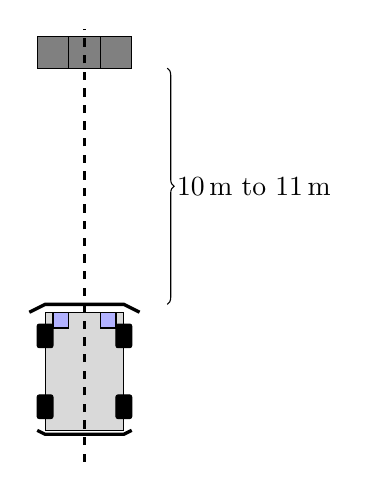
\begin{tikzpicture}
        \gokart{0}{0}{0}
    
        % Wall (three cubes)
        \draw[fill=gray] (-0.6,3) rectangle (-0.2,3.4);
        \draw[fill=gray] (-0.2,3) rectangle (0.2,3.4);
        \draw[fill=gray] (0.2,3) rectangle (0.6,3.4);
    
        % Dashed line from go-kart to wall (center axis)
        \draw[dashed, thick] (0,-2) -- (0,3.5);
    
        % Range brace annotation
        \draw [decorate, decoration = {brace, raise=10pt}] (0.7,3) -- (0.7, 0) node[pos=0.5,right=10pt,black]{\SIrange{10}{11}{\meter}};

        % Enlarged Radar sensor boxes
        \draw[fill=blue!30] (-0.4,-0.3) rectangle (-0.2,-0.1);
        \draw[fill=blue!30] (0.2,-0.3) rectangle (0.4,-0.1);
    \end{tikzpicture}
    \caption{Test scenario with dual front-mounted mmWave radar sensors.  
    This setup served as the baseline validation environment before moving to more complex scenarios.}
    \label{fig:test_scenario}
\end{figure}

\vspace{2\baselineskip}
The dual-radar arrangement increases point density and stability compared to single-radar approaches, aligning with multimodal strategies for robust state estimation \cite{Multimodal_Offroad,HighSpeed_Estimation}.  
By fusing Doppler-derived radial velocities with rotational information from the IMU, the system was designed to remain resilient in conditions where LiDAR- or camera-based odometry would degrade.  
Each radar stream was processed independently and then merged into a combined representation before entering the odometry pipeline.  

\vspace{1\baselineskip}
\paragraph*{Sub-Tasks}
The dual-radar objective implied several practical sub-tasks:  
\begin{itemize}
    \item Designing a modular pipeline to acquire and decode synchronized radar data from both sensors and the imu.  
    \item Investigating sensor configurations to balance field of view, chirp bandwidth, update rate, and detection density.  
    \item Developing mechanical mounts and selecting optimal sensor placement to ensure stability and maximize coverage.  
    \item Leveraging additional sensor information (e.g., SNR, RCS, range validity) to optimize point cloud reliability.  
    \item Employing submap aggregation to mitigate sparsity and improve stability.  
    \item Integrating Doppler velocity into the odometry estimation process.  
    \item Applying RANSAC filtering on Doppler velocities to reject dynamic points and outliers.  
    \item Implementing clustering methods to structure radar detections and isolate relevant features.  
    \item Performing ICP alignment between submaps aggregated from both sensors.  
    \item Evaluating the influence of the dual-sensor arrangement on odometry accuracy and robustness.  
    \item Validating the complete system on real-world driving scenarios.  
\end{itemize}

Taken together, these sub-tasks define the modular pipeline through which radar and IMU data are processed into ego-motion estimates.  
Each block in the pipeline corresponds to one or more of the identified tasks, from raw data acquisition and transformation, to filtering, clustering, and alignment.  
This modularity ensures that individual stages can be validated and tuned independently, while still contributing to the overall odometry framework.  
The complete processing chain is summarized in Figure~\ref{fig:dual_radar_pipeline}, which illustrates how the dual-radar inputs are merged with IMU measurements and progressively refined into robust ego-motion estimates.

\begin{figure*}[!htbp]
    \centering
    \resizebox{\textwidth}{!}{%
        \begin{tikzpicture}
            % Block style
            \tikzstyle{block} = [rectangle, draw, text width=4.5em, text centered, minimum width=6em, minimum height=4em]

            % Input branches
            \node[block] (radar1) {Radar\\Front Left};
            \node[block, below=1.2cm of radar1] (radar2) {Radar\\Front Right};

            % Physical transformation
            \node[block, right=of radar1] (transform1) {Rigid-Body\\Transform};
            \node[block, below=1.2cm of transform1] (transform2) {Rigid-Body\\Transform};

            % Merge
            \node[block, right=of transform1] (merge) {Radar Merge};

            % IMU (moved below radars)
            \node[block, below=1.2cm of transform2] (imu) {IMU};

            % Frame aggregator
            \node[block, right=of merge] (frame_aggr) {Frame\\Aggregator};
            \node[block, right=of frame_aggr] (coord_filter) {Filter\\$x,y,z$\\$\phi$, SNR};
            \node[block, right=of coord_filter] (ransac) {RANSAC};
            \node[block, right=of ransac] (doppler_filter) {Filter\\Dynamic Objects};
            \node[block, right=of doppler_filter] (clustering) {Clustering};
            \node[block, right=of clustering] (icp) {ICP};
            \node[block, right=of icp] (ego) {Ego-motion};

            % Connections
            \draw[->] (radar1) -- (transform1);
            \draw[->] (radar2) -- (transform2);
            \draw[->] (transform1) -- (merge);
            \draw[->] (transform2) -| (merge);

            % Merge and IMU both feed into Frame Aggregator
            \draw[->] (merge) -- (frame_aggr);
            \draw[->] (imu) -| (frame_aggr);

            % Continue the pipeline
            \draw[->] (frame_aggr) -- (coord_filter);
            \draw[->] (coord_filter) -- (ransac);
            \draw[->] (ransac) -- (doppler_filter);
            \draw[->] (doppler_filter) -- (clustering);
            \draw[->] (clustering) -- (icp);
            \draw[->] (icp) -- (ego);

            % Bottom brace under radar2 (dual radar inputs only)
            \draw [decorate, decoration = {brace, mirror, raise=8pt}] 
                ([xshift=-2em,yshift=-1em]radar2.south west) -- 
                ([xshift=2em,yshift=-1em]radar2.south east)
                node[midway, below=12pt] {Dual-Radar Inputs};

            % Larger bottom brace under radars and IMU
            \draw [decorate, decoration = {brace, mirror, raise=16pt}] 
                ([xshift=-2em,yshift=-8.5em]radar2.south west) -- 
                ([xshift=2em,yshift=-1em]imu.south east)
                node[midway, below=20pt] {System Sensorial Inputs};
        \end{tikzpicture}
    }
    \caption{Dual-radar pipeline showing how radar and IMU inputs are merged into the system for further processing.}
    \label{fig:dual_radar_pipeline}
\end{figure*}

\newpage
The following sections detail the hardware setup, pipeline methodology, and experimental validation.

\subsection{System Hardware}

The hardware setup combines mmWave radars, an inertial sensor, and auxiliary components into a compact test platform.  
In this section, we describe the role of each element, how they were mechanically integrated, and how the radar configuration was selected for odometry tasks.  

\vspace{0.5em}
\subsubsection{System Sensors}
\hfill
\\
The sensors that are implemented and used in this project are the following:
\vspace{0.5em}
\subsubsubsection{mmWave Radar (IWR6843AOP)}
\hfill
\\
\indent The IWR6843AOPEVM development board from Texas Instruments features the IWR6843AOP, a high performance 4D mmWave FMCW sensor with Antenna On Package (AOP) design.
Although IWR6843AOP is intended for industrial applications and its complementary chip, AWR6843AOP, for automotive applications, IWR6843AOP was used in this project because it is available in the form of this development board and the two chips are identical in terms of their functionalities, only differing in compliance with automotive  industry \cite{iwr_awr_diff}.
Its small physical size, due to its AOP design, makes it an optimal choice for the desired mounting position, the go-kart's steering column.
\begin{figure}[!htbp]
    \centering
    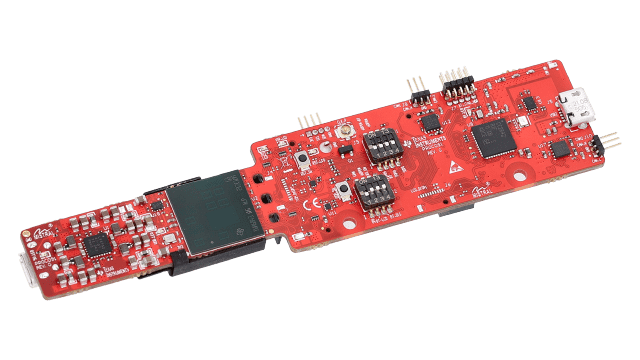
\includegraphics[width=0.7\linewidth]{images/iwr6843aopevm-angled.png}
    \caption{IWR6843AOP sensor\\
    \textit{Source: Texas Instruments, available at \url{https://www.ti.com/ds_dgm/images/fbd_swrs219f.gif}}}
    \label{fig:IWR6843AOP sensor}
\end{figure}

\par
The IWR6843AOP radar sensor operates within the frequency range of \SIrange{60}{64}{\giga\hertz} and integrates 4 receive (RX) and 3 transmit (TX) antennas, radio frequency (RF) front-end stages, analog signal processing, and digital signal processing (DSP).
It offers a wide range of communication interfaces including SPI, I2C, CAN-FD, UART and LVDS for raw data access and an Arm Cortex-R4F microcontroller for user-applications as shown in the Figure~\ref{fig:IWR6843AOP_internal} \cite{dev_board_page}.

\begin{figure}[!htbp]
    \centering
    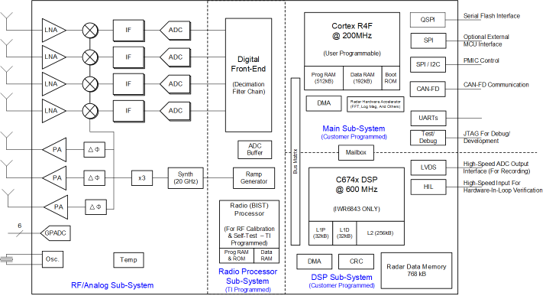
\includegraphics[width=1.0\linewidth]{images/blockdiagram.png}
    \caption{IWR6843AOP internal block diagram.\\
    \textit{Source: Texas Instruments, available at \url{https://www.ti.com/ds_dgm/images/fbd_swrs219f.gif}}}
    \label{fig:IWR6843AOP_internal}
\end{figure}

\begin{comment}
    Here create a connecto to the calibration of the sensor
\end{comment}

As some operating parameters influence each other, their selection must be done carefully while observing the influence of the trade-offs involved.
This could be referred to as "sensor tuning" and is a critical step because it directly impacts the system's accuracy and performance.

The following operating parameters can be tuned:
\begin{itemize}
    \item Frame rate
    \item Range resolution
    \item Maximum unambigious range
    \item Maximum radial velocity
    \item Radial velocity resolution
\end{itemize}

Tuning these operating parameters introduces trade-offs by influencing each other in the following ways:
\begin{table}[h]
    \centering
    \resizebox{\columnwidth}{!}{
    \begin{tabular}{|l|l|p{3.5cm}|p{3.5cm}|p{3.5cm}|}
        \hline
        \textbf{Tuning Parameter} & \textbf{Effect on Performance} & \textbf{Related HW Block} & \textbf{Trade-Off} \\
        \hline
        Frame Rate & Higher FPS = faster updates but more processing load & C674x DSP, Radar Data Memory & Higher FPS reduces maximum range \\
        \hline
        Range Resolution & Higher resolution = better object separation & ADC, 1D FFT (Range FFT) & Higher resolution reduces max range \\
        \hline
        Maximum Range & Determines farthest detectable object & RF Front-End, PA, LNA, ADC & Higher range lowers resolution \\
        \hline
        Radial Velocity Resolution & Improves speed accuracy & DSP, 2D FFT (Doppler FFT) & Higher resolution requires more chirps \\
        \hline
        Maximum Radial Velocity & Detects fast-moving objects & Chirp rate, TX Antennas, 2D FFT & Higher max velocity reduces resolution \\
        \hline
    \end{tabular}
    }
    \caption{Radar System Tuning Parameters and Trade-offs}
    \label{tab:mmWave_Sensor_Parameters}
\end{table}
The resulting overall accuracy of the velocity and distance measurements is again dependent on these operating parameters:
\begin{itemize}
\item \textbf{Radial velocity accuracy:} A fine balance between velocity resolution and frame rate must be maintained to ensure precise Doppler shift measurements. Lower resolution results in rounded velocity values, while an excessively high frame rate may introduce computational bottlenecks.
\item \textbf{Distance accuracy:} Optimizing range resolution and maximum range ensures that detected objects are positioned accurately within the environment. Increasing range often sacrifices resolution, leading to potential inaccuracies in close-range detections.
\item \textbf{Signal processing considerations:} The FFT calculation parameters directly affect both range and Doppler calculations, influencing the ability to distinguish between objects and detect small velocity variations.
\end{itemize}
\vspace{0.5em}
\subsubsubsection{Inertial Measurement Unit (IMU)}  
\hfill
\\
\indent The MTi-G-710 from Xsens is a high-performance GNSS/INS module that integrates a 3D accelerometer, 3D gyroscope, 3D magnetometer, and barometer with an onboard GNSS receiver.  
Although designed as a complete navigation unit capable of delivering position and velocity estimates, in this project it was used specifically for its orientation outputs, provided in the form of quaternions, Euler angles, or rotation matrices \cite{mti710_manual}.  
Its compact form factor and proven sensor-fusion engine made it a suitable choice for integration into the test platform, complementing the radar subsystem by supplying real-time orientation references.  

For the present setup, the device was configured to output quaternions, as this representation avoids singularities inherent in Euler angles and provides numerical stability for continuous tracking.  
These quaternions were used to track the vehicle attitude and to align radar point clouds within a consistent vehicle-centric coordinate frame.  
By relying on the MTi-G-710 internal fusion engine rather than implementing custom filtering, the system leveraged factory-calibrated algorithms for bias correction and drift reduction, minimizing processing overhead on the host platform.  

To interface with the device and parse its MTData2 protocol, an open-source implementation from Scottapotamas was adopted \cite{xsens_repo}.  
This repository enabled robust packet parsing and quaternion extraction in Python, ensuring seamless integration of the IMU data stream into the radar processing pipeline.  

\begin{figure}[!htbp]
    \centering
    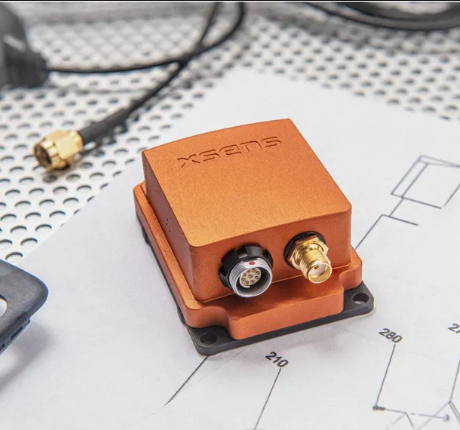
\includegraphics[width=0.65\linewidth]{images/mti_g710.png}
    \caption{MTi-G710 high-performance inertial navigation system (INS).\\
    \textit{Source: Movella, available at \url{https://www.movella.com/sensor-modules/xsens-mti-7-gnss-ins}}}
    \label{fig:MTi-G710 sensor}
\end{figure}

\subsubsubsection{Webcam}
\hfill
\\
\indent A Logitech C270 HD webcam was included in the experimental platform for the sole purpose of video recording.  
Unlike the radar and IMU, the camera was not integrated into the sensing or processing pipeline and did not contribute any data to the odometry estimation system.  
Its role was limited to providing visual documentation of the test environment, allowing experiments to be reviewed and contextualized with synchronized video footage.  

\vspace{0.5em}
\subsubsection{Mechanical Integration}
\hfill
\\
\indent The mechanical design and integration of the sensing suite were crucial to ensure stable operation, accurate data alignment, and reproducibility across experiments. 
This subsection is divided into three parts:
\begin{itemize}
    \item 3D printed mounts for flexible radar positioning.  
    \item 3D dedicated IMU mounting plate.  
    \item Geometric placement of radars and corresponding coordinate transformations.  
\end{itemize}

\vspace{0.5em}
\paragraph{Radar Mounting Design}
\hfill
\\
% -- Explain the custom 3D-printed designs that allowed adjustable yaw/pitch positioning of the radars.
% -- Show figures of the mounts and describe their role in fine-tuning sensor orientation.
% -- Emphasize stability and repeatability.
\indent A standard mounting bracket is provided by the manufacturer for the IWR6843AOP sensor, as shown in Figure~\ref{fig:IWR6843AOP_mount}. 
While suitable for simple setups, this bracket only allows a fixed mounting position without the possibility of adjusting yaw or pitch. 
Such limitations restrict the ability to optimize the radar field of view for different vehicle placements and test scenarios.  

To overcome this, a custom 3D-printed bracket was developed, enabling adjustable tilt and offering greater flexibility in sensor alignment (Figures~\ref{fig:IWR6843AOP_mounts_comparison} and \ref{fig:IWR6843AOP_3D_mounts}). 
This design provides precise control over the radar orientation, which is essential for minimizing ground reflections, extending horizontal coverage, and ensuring that both radars could be consistently aligned with the vehicle’s coordinate frame.  
\newpage
The bracket consists of three main components:  
\begin{itemize}
    \item A stable \textbf{mounting base} securely attached to the vehicle platform.  
    \item A \textbf{sensor frame} that holds the IWR6843AOP in position.  
    \item An adjustable \textbf{tightening screw} that locks the tilt angle once aligned.  
\end{itemize}

The mounts were fabricated using PLA, chosen for its ease of printing and adequate stiffness for field use. 
They were fixed to the vehicle platform with hot glue, a lightweight yet sufficiently rigid method to ensure stability during operation. 
This approach minimized vibration-induced artifacts and guaranteed repeatable positioning across experiments.  

By introducing this adjustable design, the system achieved both mechanical robustness and alignment flexibility, enabling more accurate calibration of the dual-radar setup and improving consistency in downstream data fusion.  

\begin{figure}[!htbp]
    \centering
    \begin{subfigure}[t]{0.48\linewidth}
        \centering
        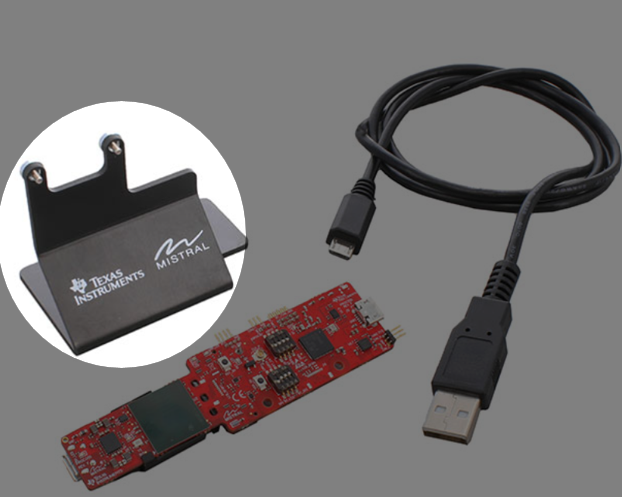
\includegraphics[width=\linewidth]{images/IWR6843Mount.png}
        \caption{Manufacturer-provided mount for the IWR6843AOP sensor. This design fixes the sensor in place without tilt adjustment, limiting flexibility.\\
        \textit{Source: amicus engineering, available at \href{https://amicus.com.sg/products/iwr6843aop-evaluation-module-for-single-chip-60ghz-antenna-on-package-aop-mmwave-sensor/}{amicus.com.sg}}}
        \label{fig:IWR6843AOP_mount}
    \end{subfigure}
    \hfill
    \begin{subfigure}[t]{0.48\linewidth}
        \centering
        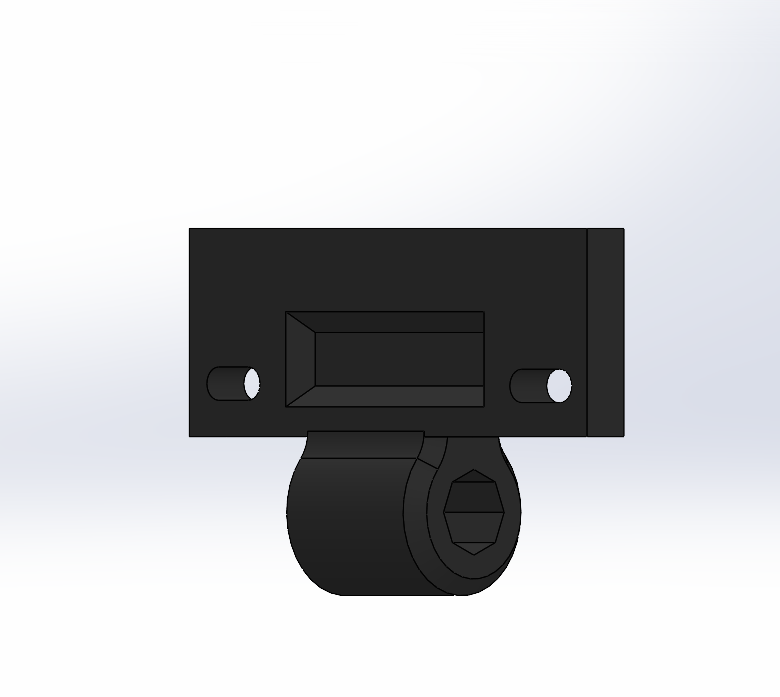
\includegraphics[width=\linewidth]{images/3DModelSensorMount.png}
        \caption{Custom 3D-printed mount designed. It enables controlled tilt adjustments, ensuring repeatable alignment and optimized field of view.}
        \label{fig:IWR6843AOP_3D_sensorMount}
    \end{subfigure}
    \caption{Comparison of sensor mounting options for the IWR6843AOP radar: (a) fixed manufacturer mount and (b) adjustable 3D-printed design. The custom bracket provides alignment flexibility and stability, improving calibration for dual-radar operation.}
    \label{fig:IWR6843AOP_mounts_comparison}
\end{figure}

\begin{figure}[!htbp]
    \centering
    \begin{subfigure}[t]{0.48\linewidth}
        \centering
        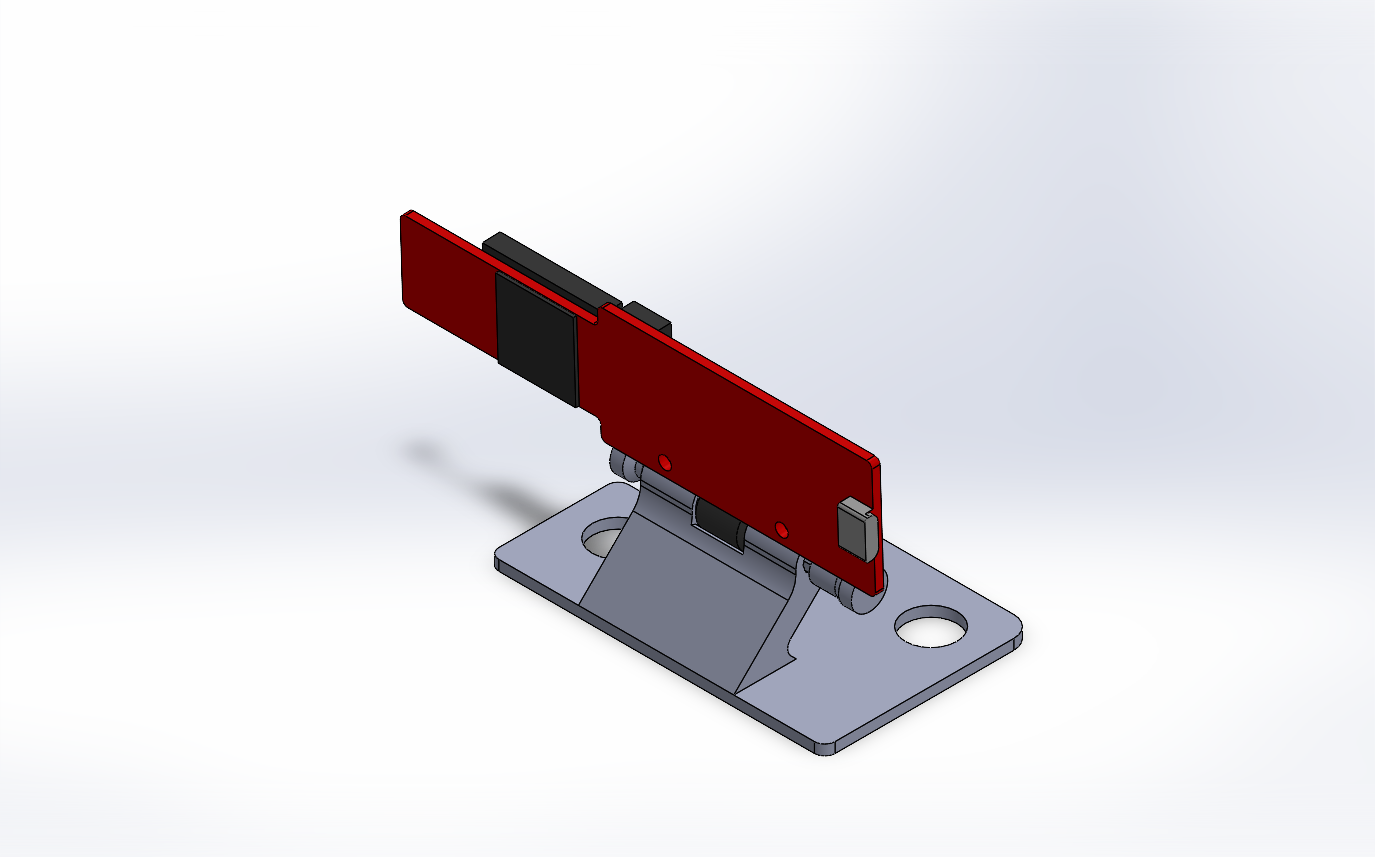
\includegraphics[width=\linewidth]{images/3DModelFullSensor.png}
        \caption{IWR6843AOP sensor mounted on the custom 3D-printed bracket in its default upright orientation. 
        The mount provides a stable base while allowing tilt adjustments.}
        \label{fig:IWR6843AOP_3D_mount}
    \end{subfigure}
    \hfill
    \begin{subfigure}[t]{0.48\linewidth}
        \centering
        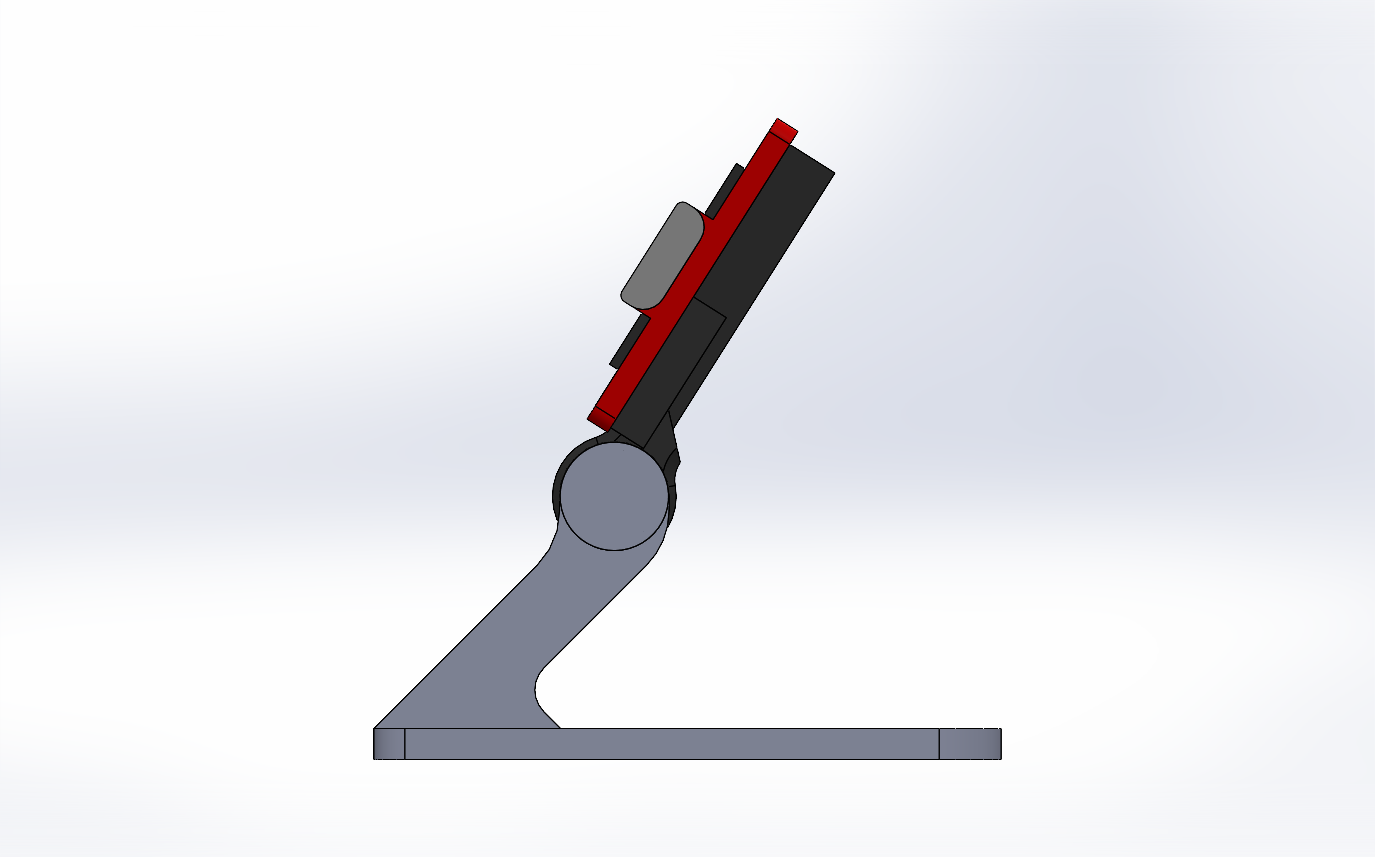
\includegraphics[width=\linewidth]{images/3DModelFullSensorSideTilt.png}
        \caption{Side view showing the tilt functionality of the custom bracket. 
        This adjustability was critical for compensating the $15^\circ$ upward tilt used in the dual-radar configuration.}
        \label{fig:IWR6843AOP_3D_mount_tilt}
    \end{subfigure}
    \caption{Implementation of the custom 3D-printed mounting solution for the IWR6843AOP radar. 
    The design combines stability with controlled tilt adjustment, enabling repeatable calibration and improved alignment with the vehicle frame.}
    \label{fig:IWR6843AOP_3D_mounts}
\end{figure}

\begin{figure}[!htbp]
    \centering
    \includegraphics[width=0.65\linewidth]{images/SensorInVehicle.png}
    \caption{Prototype installation of the IWR6843AOP radar sensor on the vehicle. 
    This early mounting solution was used for visualization and comparison with the 3D design, but it was not adopted as the final configuration.}
    \label{fig:SensorInVehicle}
\end{figure}

While the 3D model (Figures~\ref{fig:IWR6843AOP_mounts_comparison}-\ref{fig:IWR6843AOP_3D_mounts}) illustrates the intended mounting geometry, Figure~\ref{fig:SensorInVehicle} shows an intermediate real-world implementation.
This prototype installation provided a practical check of sensor tilt and positioning but was later replaced by the custom 3D-printed bracket, which ensured stability, repeatability, and precise control over yaw and pitch adjustments.

\vspace{0.5em}
\paragraph{IMU Mounting Design}
\hfill
\\
\indent The MTi-G710 IMU required a stable and horizontally aligned installation point to ensure that its quaternion orientation output could be directly mapped to the vehicle reference frame without introducing additional correction.  
To achieve this, a custom mounting solution was developed, illustrated in Figure~\ref{fig:MTi3DModel}.  

\vspace{3\baselineskip}
The 3D design, shown in Figure~\ref{fig:MTi3DModel}, highlights the three main elements of the assembly:  
\begin{enumerate}
    \item The MTi-G710 sensor.  
    \item A flat mounting plate designed to secure the device.  
    \item The rear vehicle mounting spot, located near the spoiler.  
\end{enumerate}

This location was selected because it provided a rigid and vibration-resistant base, while also being naturally aligned with the horizontal plane of the vehicle.  
The design ensured that the IMU could be mounted flush, minimizing installation errors and avoiding unnecessary post-processing of orientation data.  

The real-world implementation is shown in Figure~\ref{fig:MTiRealMount}, where the IMU was securely fixed to the vehicle.  
This placement offered both ease of integration and the stable reference needed for reliable sensor fusion with the radar system.  

\begin{figure}[!htbp]
    \centering
    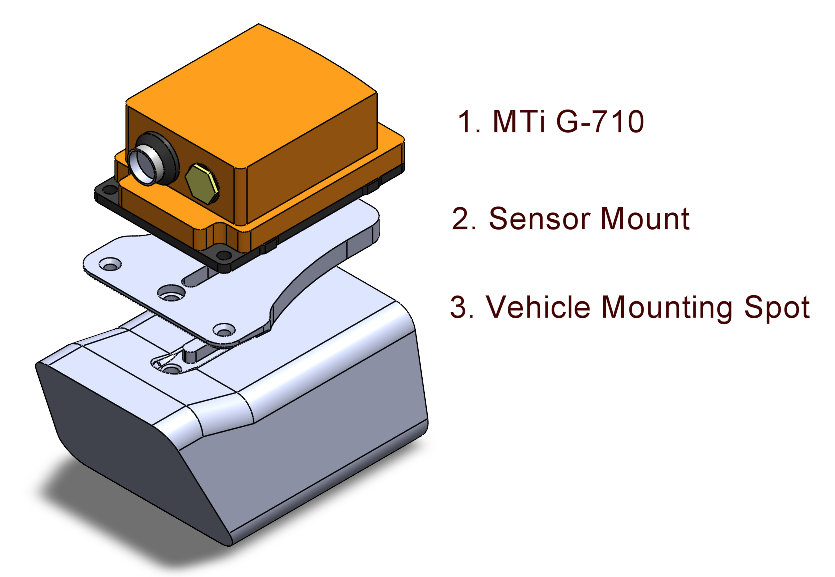
\includegraphics[width=0.65\linewidth]{images/MTi3DModel.png}
    \caption{3D model of the MTi-G710 IMU installation. 
    The design consists of (1) the IMU, (2) a custom flat sensor mount, and (3) the rear vehicle mounting spot selected for its stability and horizontal alignment.}
    \label{fig:MTi3DModel}
\end{figure}

\begin{figure}[!htbp]
    \centering
    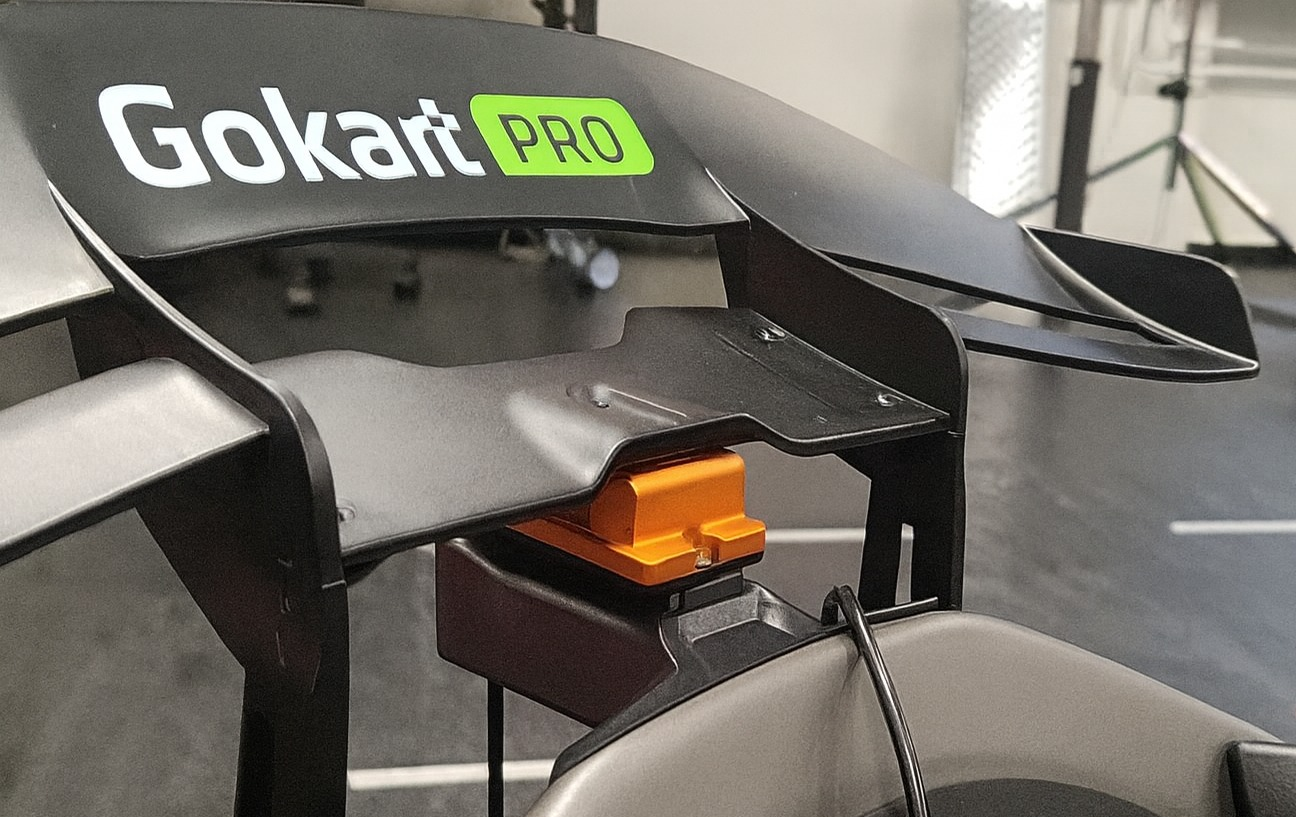
\includegraphics[width=0.65\linewidth]{images/MTiVehicleMount.png}
    \caption{Real-world installation of the MTi-G710 at the rear vehicle mount point. 
    This position near the spoiler ensured a rigid and level platform, reducing post-processing requirements for orientation correction.}
    \label{fig:MTiRealMount}
\end{figure}

\newpage
\subsubsection{Sensor Setup and Calibration}
\hfill
\\
\indent An understanding of how the sensors operate is required before they can be correctly integrated into the system.  
This involves studying their configuration tools, calibration procedures, and data output formats.  
Only by understanding their internal operation and limitations can they be properly adapted for the precise requirements of this application.

\vspace{0.5em}
\noindent\textbf{Radar Setup and Calibration}
\label{sec:radar_setup_calibration}
\vspace{0.5em}

\paragraph{Configuration Tools}
\hfill
\\
\indent To configure and validate the radar sensors, two official Texas Instruments tools were employed: the \textit{mmWave Demo Visualizer} and the \textit{mmWave Sensing Estimator}.  
These tools allowed the rapid prototyping of chirp profiles and provided immediate feedback on their impact on range and velocity performance.  

The \textbf{mmWave Demo Visualizer} \cite{mmwave_demo_web, mmwave_demo_doc} is a browser-based application that enables basic sensor configuration and visualization.  
It allows the user to adjust frame rate, range resolution, maximum range, and velocity settings, while simultaneously observing output plots such as point clouds, noise profile, range profile, and Doppler heatmaps.  
This tool was particularly useful for testing standard chirp configurations and ensuring the correct operation of the radar hardware in a controlled environment.  
Figure~\ref{fig:mmwave_demo_visualizer} shows an example of the configuration interface.  

\begin{figure}[!htbp]
    \centering
    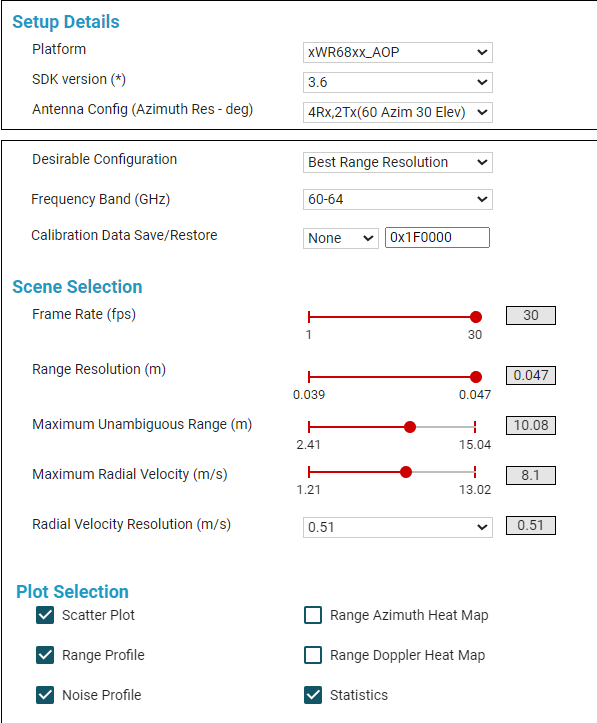
\includegraphics[width=0.9\linewidth]{images/mmWaveDemoVisualizer.png}
    \caption{mmWave Demo Visualizer interface for radar setup and visualization.\\
    \textit{Source: Texas Instruments, available at \href{https://dev.ti.com/gallery/view/mmwave/mmWave_Demo_Visualizer/ver/3.6.0/}{dev.ti.com}}}
    \label{fig:mmwave_demo_visualizer}
\end{figure}

Complementing this, the \textbf{mmWave Sensing Estimator} \cite{mmwave_demo_output} provides a theoretical framework to design chirp profiles.  
By specifying parameters such as slope, bandwidth, ADC sampling rate, and frame timing, the tool outputs derived radar capabilities including range resolution, maximum detectable velocity, and unambiguous range.  
However, it must be emphasized that the estimator only generates feasible profiles. However, it does not guarantee hardware compatibility.  
Each configuration must be tested on the actual radar device to confirm correct execution.  
Figure~\ref{fig:mmwave_sensing_estimator} illustrates the chirp design interface of the estimator.  

\begin{figure}[!htbp]
    \centering
    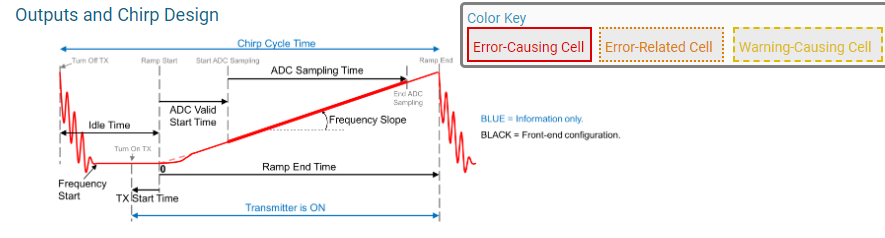
\includegraphics[width=0.9\linewidth]{images/sensingEstimatorChirp.png}
    \caption{mmWave Sensing Estimator interface for chirp configuration design.\\
    \textit{Source: Texas Instruments, available at \href{https://dev.ti.com/gallery/view/mmwave/mmWaveSensingEstimator/ver/2.5.1/}{dev.ti.com}}}
    \label{fig:mmwave_sensing_estimator}
\end{figure}

\vspace{0.5em}
\paragraph{Chirp Configuration}
\hfill
\\
\indent The IWR6843AOP operates as a Frequency-Modulated Continuous Wave (FMCW) radar, transmitting chirps whose frequency increases linearly over a bandwidth $B$ during a duration $T_c$.  
Reflected signals return with a frequency shift that encodes target range, while Doppler shifts across successive chirps provide relative velocity.  

The chirp is defined by:
\begin{itemize}
    \item Start frequency $f_0$ [GHz]
    \item Frequency slope $S$ [MHz/$\mu$s]
    \item Chirp duration $T_c$ [$\mu$s]
    \item Idle time between chirps $T_{\text{idle}}$ [$\mu$s]
    \item Sampling rate $f_s$ [Msps]
    \item Bandwidth $B = S \cdot T_c$ [MHz]
\end{itemize}
From these parameters, the sensing performance is determined as:
\[
    \Delta R = \frac{c}{2B} \ [\text{m}], \qquad
    R_{\max} = \frac{c f_s}{2S} \ [\text{m}],
\]
\[
    \Delta v = \frac{\lambda}{2 N_c T_c} \ [\text{m/s}], \qquad
    v_{\max} = \frac{\lambda}{4 T_c} \ [\text{m/s}],
\]
where $\Delta R$ is \textbf{range resolution}, $R_{\max}$ the \textbf{maximum unambiguous range}, $\Delta v$ the \textbf{velocity resolution}, and $v_{\max}$ the \textbf{maximum unambiguous velocity}.  

\textbf{Full-Bandwidth Chirp (Single 4 GHz Sweep)}, shown in Fig.~\ref{fig:profile4GHz}, provides the finest possible range resolution by sweeping the entire 4~GHz spectrum in a single chirp.  
This configuration is well suited for precise spatial localization but requires high ADC sampling rates and is more prone to interference, making it practical mainly for single-radar setups.  

\begin{figure}[!htbp]
    \centering
    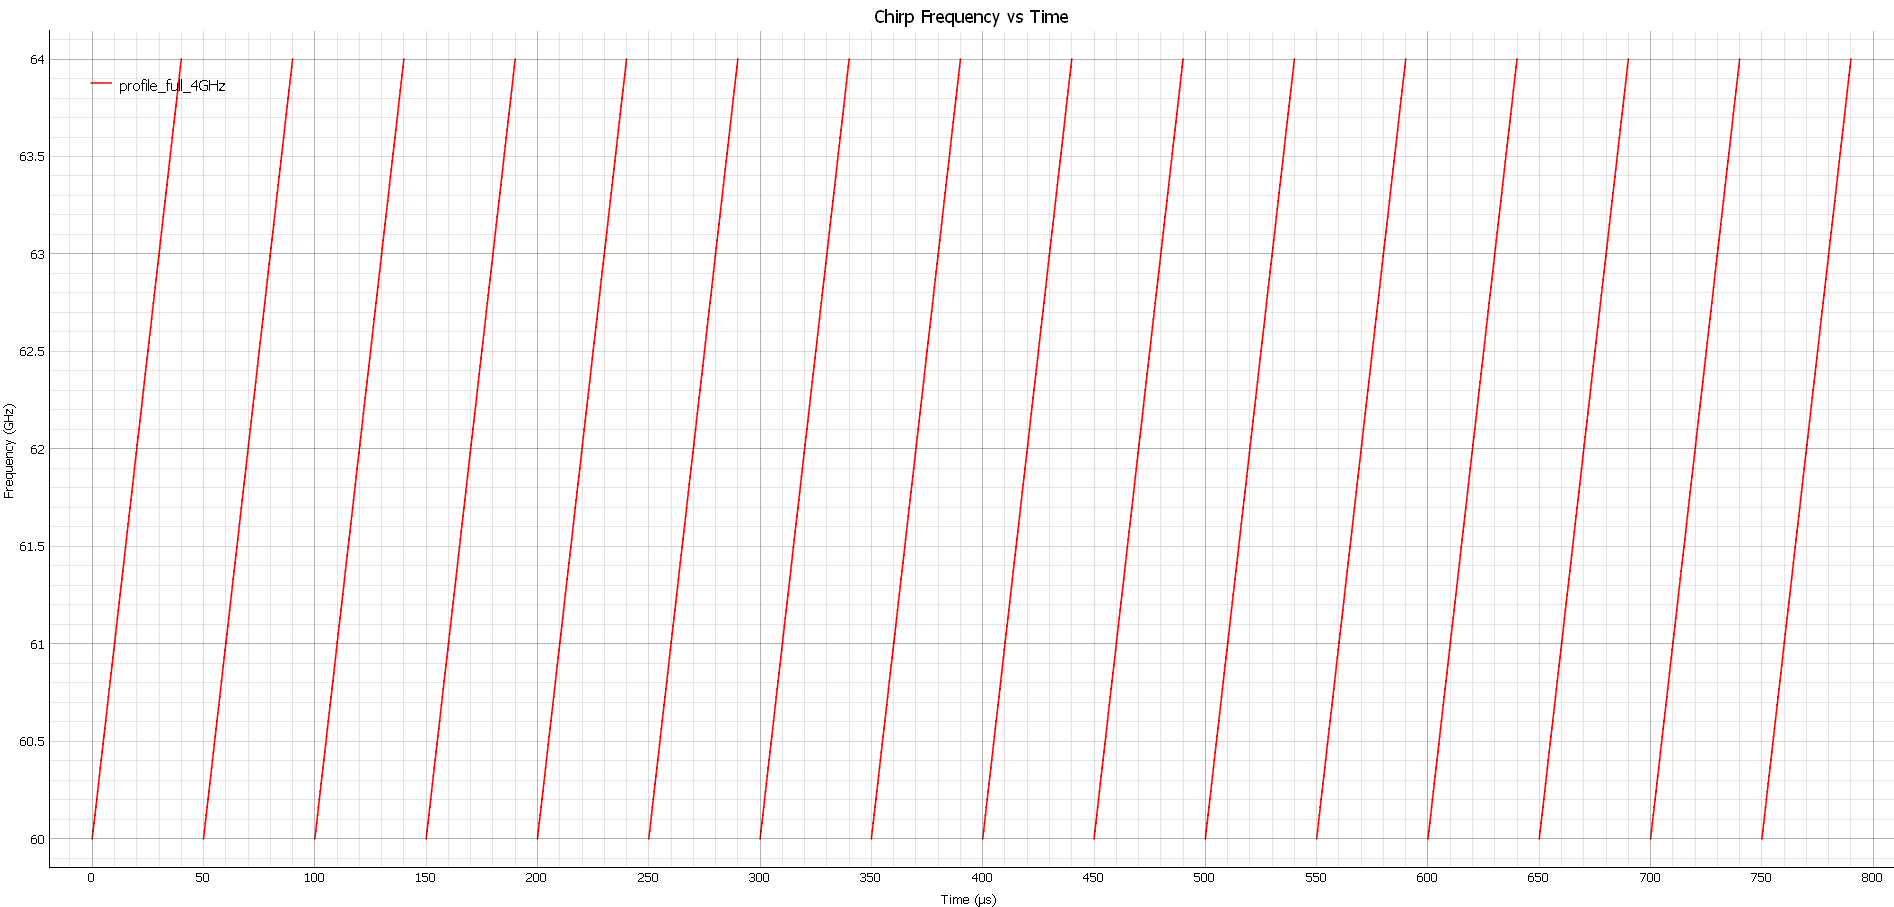
\includegraphics[width=0.7\linewidth]{images/profile_full_4GHz.png}
    \caption{Full-bandwidth chirp (single 4~GHz sweep).  
    \textit{Source: Texas Instruments, available in mmWave Demo Visualizer \cite{mmwave_demo_doc}}}
    \label{fig:profile4GHz}
\end{figure}

\textbf{Divided-Bandwidth Chirps (Two 2~GHz Sweeps)}, shown in Fig.~\ref{fig:profile2GHz}, split the 4~GHz spectrum into two 2~GHz chirps.  
Although this reduces range resolution compared to a full-band sweep, it lowers ADC requirements and enables reliable operation of dual-radar systems.  

In this setup, one chirp configuration was assigned to each radar (Config~A $\rightarrow$ Radar~A, Config~B $\rightarrow$ Radar~B).  
By operating on distinct frequency ranges, the radars avoided spectral overlap, preventing ghost targets and preserving point cloud quality.  

\begin{figure}[!htbp]
    \centering
    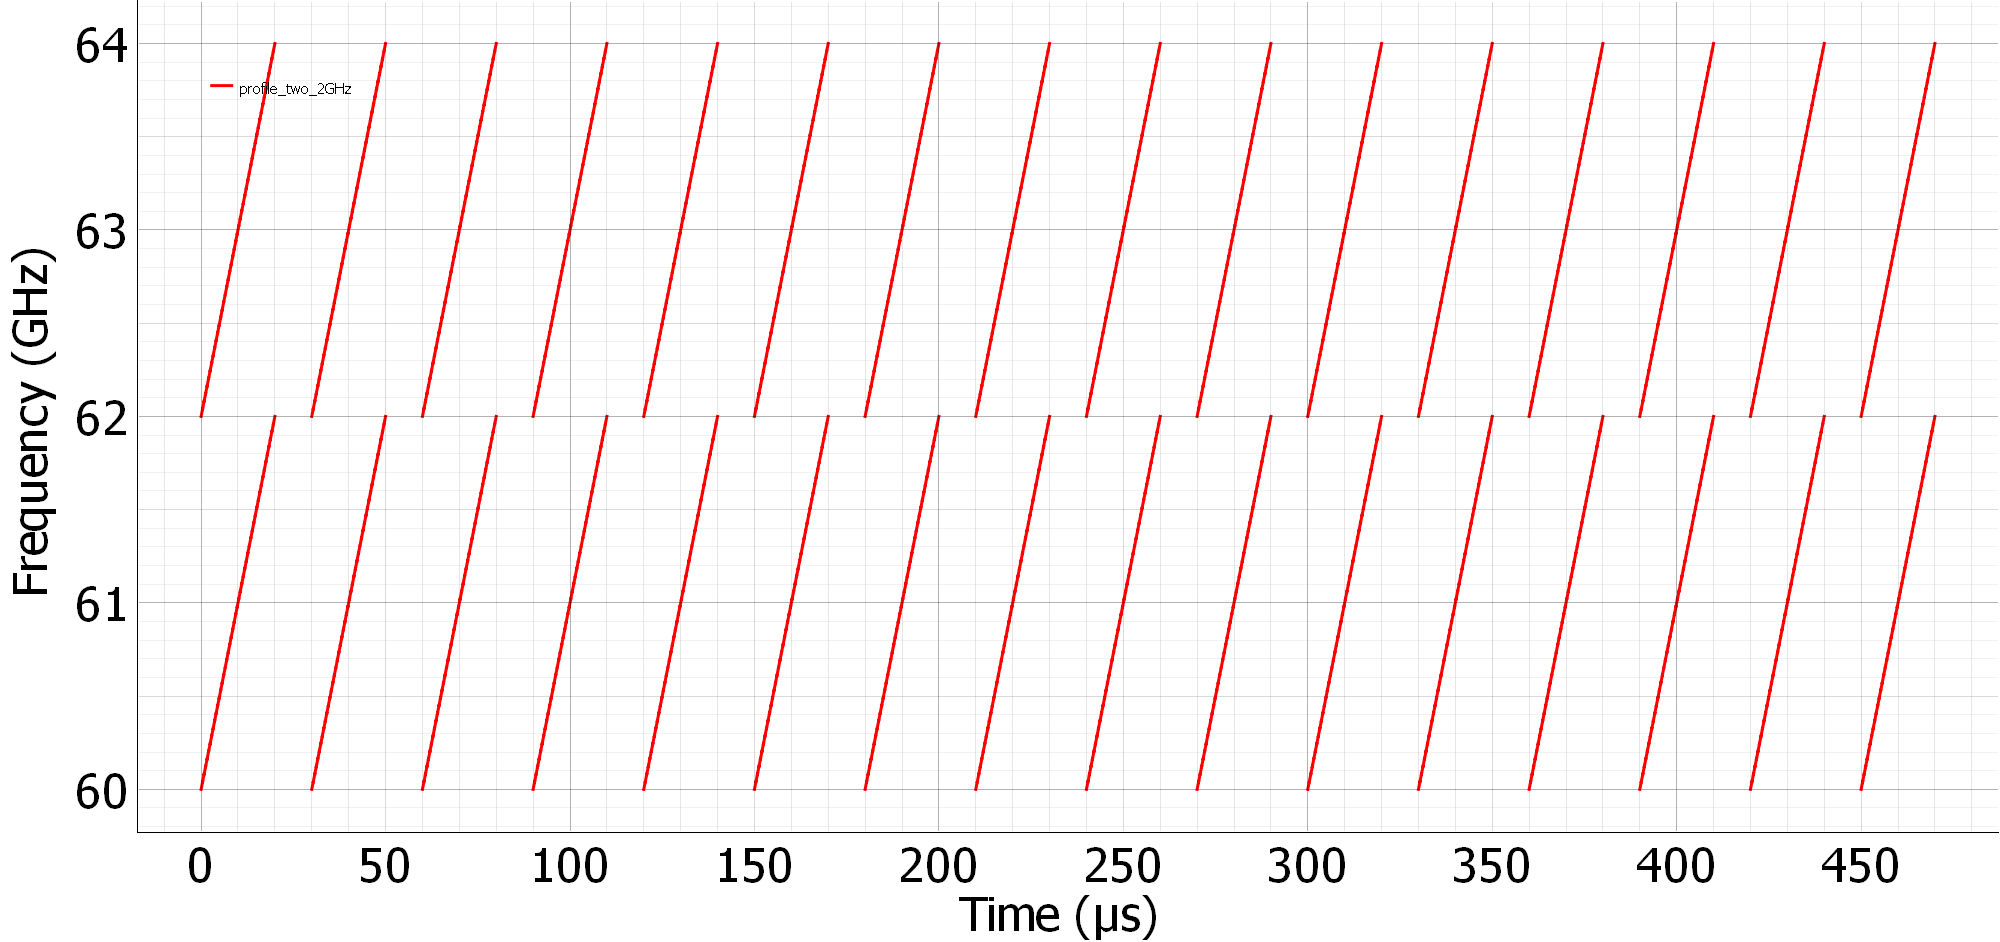
\includegraphics[width=0.7\linewidth]{images/profile_two_2GHz.png}
    \caption{Divided-band chirps (two 2~GHz sweeps).  
    \textit{Source: Texas Instruments, available in mmWave Demo Visualizer \cite{mmwave_demo_doc}}}
    \label{fig:profile2GHz}
\end{figure}

The final parameters were derived using the \textit{mmWave Sensing Estimator} tool \cite{mmwave_demo_output}.  
The divided-band strategy provided a balanced trade-off between resolution and robustness, ensuring stable dual-radar operation while avoiding the interference issues inherent to full-bandwidth sweeps.

\textbf{Same-Band Chirps (Interference Case)} — Using identical chirp configurations on both radars introduced strong mutual interference, which was expected in theory but validated here through practical testing.  
For example, in the vehicle-pushing test (Fig.~\ref{fig:dual_samechirp_pointcloud}) and in the walking-person case (Fig.~\ref{fig:dual_samechirp_cluster}), detections appeared artificially expanded or distorted compared to what was expected, with a single person spanning nearly \SI{3}{\meter}.  
While this spatial deformation was visible in the point clouds, the RANSAC analysis (Fig.~\ref{fig:dual_samechirp_ransac}) provided clearer evidence of the interference, with estimated radial velocities reaching up to $\pm$\SI{5}{\meter\per\second} despite the slow and controlled motions.  
This underlines that the main strength of the radar lies in the Doppler information extracted from detections, which in this case exposed the interference effects more clearly than the point cloud itself.  

These inconsistencies confirm that cross-talk affects both point cloud density and Doppler-based velocity estimation, making odometry unreliable.  
This experiment demonstrated the necessity of separating chirp frequency bands, leading to the adoption of the divided-bandwidth configuration for stable dual-radar operation.

\begin{figure}[!htbp]
    \centering
    \begin{subfigure}{0.48\linewidth}
        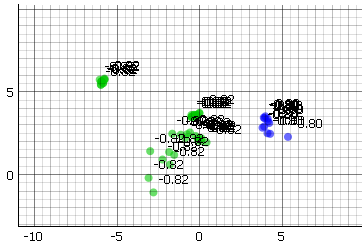
\includegraphics[width=\linewidth]{images/DualSensorSameConfigPointCloud.png}
        \caption{Point cloud of the vehicle-pushing scenario.}
        \label{fig:dual_samechirp_pointcloud}
    \end{subfigure}
    \hfill
    \begin{subfigure}{0.48\linewidth}
        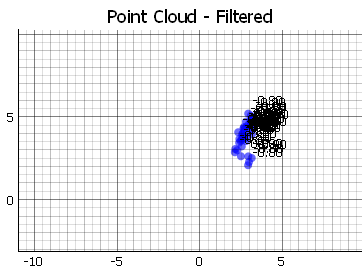
\includegraphics[width=\linewidth]{images/DualSensorSameConfigPointCloudPerson.png}
        \caption{Point cloud of the walking-person scenario.}
        \label{fig:dual_samechirp_cluster}
    \end{subfigure}
    \caption{Point clouds from dual-radar interference with same-band chirps (green = Radar~A, blue = Radar~B).  
    Scenario (a) corresponds to pushing the vehicle, and (b) to a person walking towards the vehicle.}
    \label{fig:dual_samechirp_results}
\end{figure}

\begin{figure}[!htbp]
    \centering
    \begin{subfigure}{0.48\linewidth}
        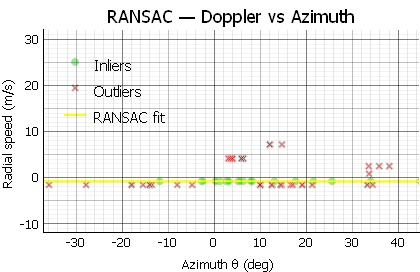
\includegraphics[width=\linewidth]{images/DualSensorSameConfigRansac.png}
        \caption{RANSAC of scenario (a) from Fig.~\ref{fig:dual_samechirp_results}.}
        \label{fig:dual_samechirp_ransac_vehicle}
    \end{subfigure}
    \hfill
    \begin{subfigure}{0.48\linewidth}
        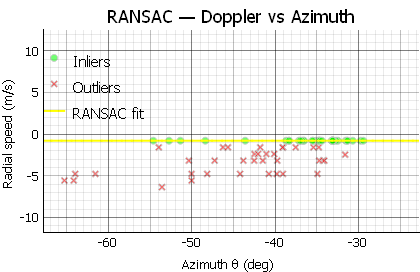
\includegraphics[width=\linewidth]{images/DualSensorSameConfigPersonRansac.png}
        \caption{RANSAC of scenario (b) from Fig.~\ref{fig:dual_samechirp_results}.}
        \label{fig:dual_samechirp_ransac_person}
    \end{subfigure}
    \caption{RANSAC Doppler vs.\ Azimuth for the same-band chirp cases.  
    Both confirm that interference causes incorrect velocity estimates when both radars share the same chirp band.}
    \label{fig:dual_samechirp_ransac}
\end{figure}

\newpage
\noindent\textbf{IMU Setup and Calibration}
\label{sec:imu_setup_calibration}

\setcounter{paragraph}{0} % Restart paragraph numbering

\paragraph{Configuration Tools}
\hfill
\\
The MTi-G-710 was first evaluated with \textit{Xsens MT Manager} to understand the sensor outputs and axis conventions.  
Using the tool, quaternion orientation was visualized in real time while the unit was held still and under gentle rotations to verify stability and drift.  
Reference frames were checked so that the IMU heading and gravity vector aligned with the vehicle-centric frame used in the radar pipeline.  
Output rate, message content, and quaternion format were confirmed in this stage before any integration work.  
This step served only for validation and sanity checks; the final system consumed the IMU stream directly during experiments.  
\vspace{0.5em}
\paragraph{Calibration Aspects}
\hfill
\\
The IMU was mounted on a rigid, nearly horizontal plate at the rear of the vehicle to minimize vibrations and to avoid introducing tilt that would require post-processing.  
On power-up, the device was initialized with a short configuration sequence to enable quaternion output at the desired rate, as specified in the low-level protocol documentation~\cite{mti_lowlevel_doc}.  
This sequence places the device in configuration mode, sets the output configuration (quaternions at a fixed sample rate), and returns it to measurement mode for streaming.  
Because the MTi-G-710 is factory-calibrated and runs an internal sensor-fusion engine, no additional field calibration was required beyond correct mounting and a stable magnetic/metal environment~\cite{mti710_manual}.  
GNSS and velocity outputs were not used in this work; only quaternions were consumed to provide a reliable attitude reference for aligning radar point clouds.  

\section{Processing Pipeline}
\label{sec:processing_pipeline}

Having defined the system hardware and sensor configurations, the next step is to establish the processing methodology that transforms raw sensor outputs into reliable odometry estimates.  
The proposed pipeline follows a modular structure, where each stage addresses a specific task: aligning radar frames through rigid-body transformations, merging dual-sensor data, filtering unreliable detections, clustering meaningful structures, and finally estimating ego-motion using Iterative Closest Point (ICP).  

The overall data flow is illustrated in Fig.~\ref{fig:dual_radar_pipeline}, which summarizes how radar and IMU measurements are progressively refined before contributing to odometry estimation.  
This organization enables stepwise validation, as each module can be evaluated independently before integration into the complete system.  

The following subsections present the mathematical formulations and algorithmic logic of each module in detail, supported by block diagrams to illustrate the transformations applied at each stage.  
By combining radar Doppler measurements with orientation inputs from the IMU, the pipeline is designed to deliver odometry estimations even in environments where conventional vision-based or LiDAR-based methods fail.

\vspace{0.5em}
\subsection{Rigid-Body Transformation}  

Each radar sensor in the dual-radar configuration is physically mounted with a specific orientation and tilt relative to the vehicle's forward direction.
To ensure a common frame of reference for all points, it is necessary to compensate for:

\begin{itemize}
    \item \textbf{Yaw rotation}: due to angled placement ($\pm30^\circ$) of the radar modules.
    \item \textbf{Pitch tilt}: due to upward mounting tilt ($-15^\circ$), which must be compensated to recover vertical geometry.
    \item \textbf{Sensor offset}: due to the physical separation of the radar sensors in the horizontal axis (X-axis).
\end{itemize}

The transformation from radar to vehicle coordinates is expressed as:

\begin{equation}
T_{\text{veh}} = R_{\text{yaw}} \cdot R_{\text{pitch}} \cdot \vec{p}_{\text{radar}} + \vec{T}
\label{eq:radar_to_vehicle_transform}
\end{equation}

Where:
\begin{itemize}
    \item \( \vec{p}_{\text{radar}} \) is a radar point in sensor coordinates.
    \item \( R_{\text{yaw}} \) is a 2D rotation around the vertical axis ($\pm30^\circ$).
    \item \( R_{\text{pitch}} \) corrects for the upward sensor tilt ($-15^\circ$).
    \item \( \vec{T} \) is the translation vector.
\end{itemize}

These corrections ensured that detections from both radars overlapped coherently, avoiding duplicated or misaligned clusters.  
Without them, raw dual-sensor data appeared inconsistent, particularly when fusing Doppler-based velocity estimates.  
After applying yaw, pitch, and translation adjustments, the fused point cloud served as a stable input for clustering, odometry, and tracking.

\vspace{0.5em}
\subsubsection{Yaw Correction (Z-axis Rotation)}
The radar sensors are rotated relative to the vehicle frame:

\begin{itemize}
    \item Radar A (Left): Mounted at $+30^\circ$ yaw $\Rightarrow$ compensated with $-30^\circ$ rotation.
    \item Radar B (Right): Mounted at $-30^\circ$ yaw $\Rightarrow$ compensated with $+30^\circ$ rotation.
\end{itemize}

The 2D rotation in the XY-plane is defined as:
\[
\begin{bmatrix}
x' \\
y' \\
z'
\end{bmatrix}
=
\begin{bmatrix}
\cos(\theta) & -\sin(\theta) & 0 \\
\sin(\theta) & \cos(\theta) & 0 \\
0 & 0 & 1
\end{bmatrix}
\begin{bmatrix}
x \\
y \\
z
\end{bmatrix}
\]

where $\theta = \pm30^\circ$ depending on the sensor.

\begin{figure}[!htbp]
    \centering
    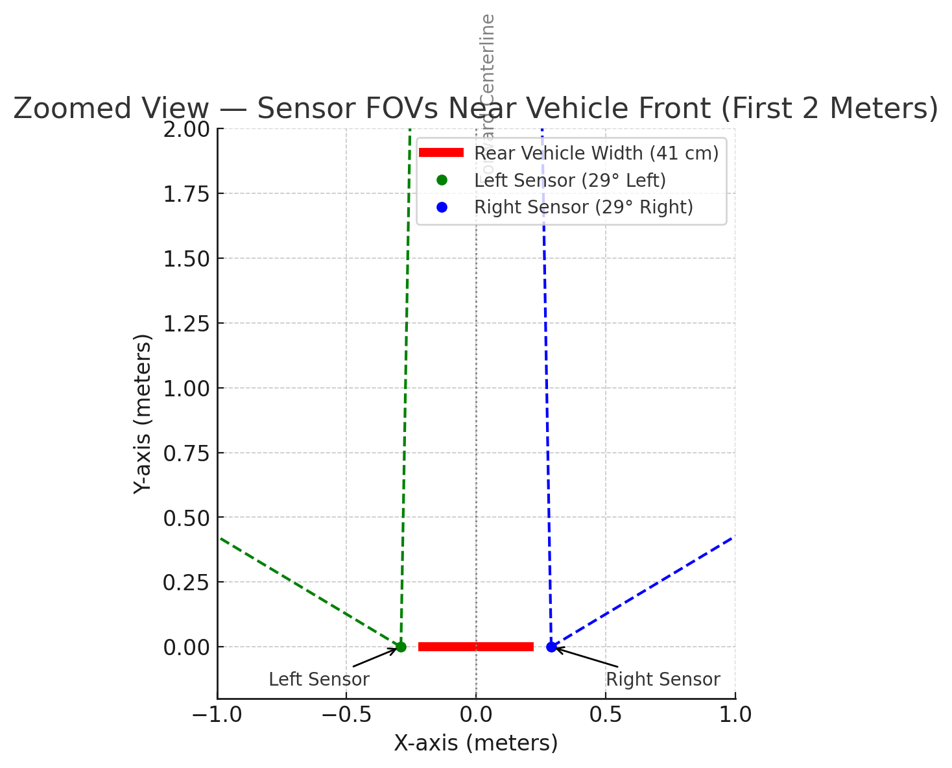
\includegraphics[width=0.8\linewidth]{images/SensorsRotation.png}
    \caption{Simulation of yaw rotation of sensors around the Z-axis ($\pm30^\circ$).}
    \label{fig:z_axis_rotation}
\end{figure}

\begin{figure}[!htbp]
    \centering
    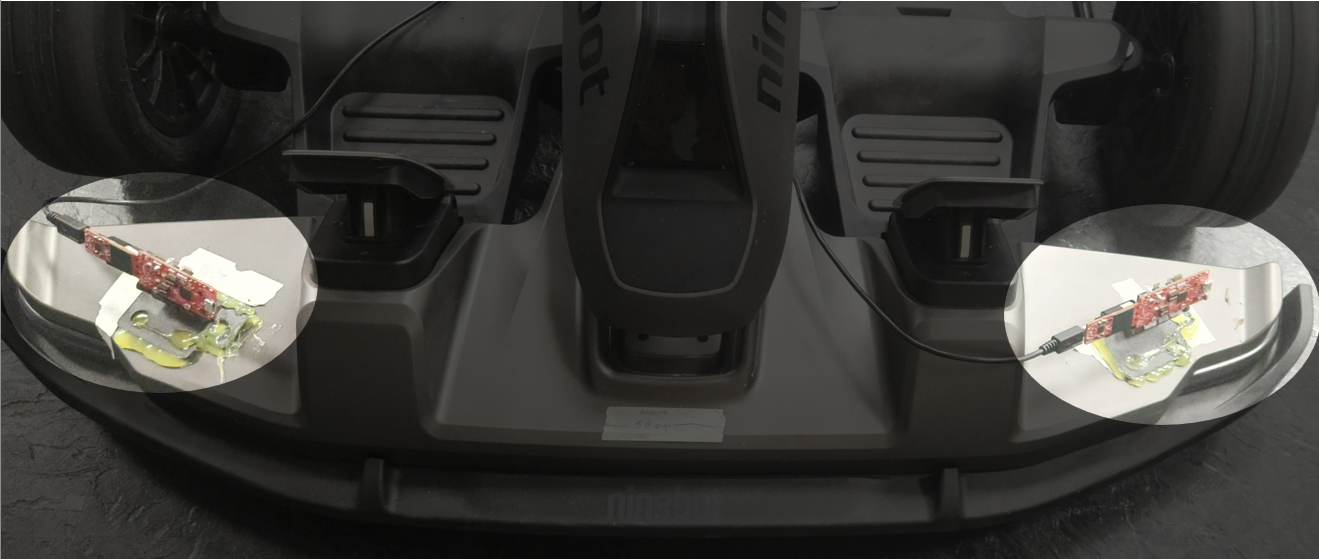
\includegraphics[width=0.8\linewidth]{images/vehicleRadarYawRotationHighlited.png}
    \caption{Real-world implementation of yaw rotation in the vehicle.}
    \label{fig:vehicleRadarYawRotation}
\end{figure}

The yaw angles of $\pm30^\circ$ were selected through a combination of physical measurement and simulation of the sensor field of view (FOV).  
Using the vehicle chassis centerline as a reference, the mounted sensors were visually measured to exhibit a yaw of approximately $28$--$32^\circ$ outward (see Fig.~\ref{fig:vehicleRadarYawRotation}), which confirmed the intended target of $30^\circ$ centered opening from the vehicle center.  
This estimate was further cross-checked in simulation by plotting the radar FOV using the TI Demo Visualizer, which allows configuration of the theoretical horizontal FOV from its default $90^\circ$ down to $60^\circ$ or $30^\circ$ respectfully.  
\begin{comment}
    Add picture of this validation
\end{comment}
The $60^\circ$ configuration was adopted as it provides improved angular resolution while discarding irrelevant detections outside the useful sector.  
Within this setting, the $\pm30^\circ$ centered mounting maximizes the combined coverage of the dual-radar system, while creating a small blind zone of approximately $4$~m directly in front of the vehicle.  
This trade-off was deliberately accepted to ensure the widest effective overlap of both radars for odometry tasks.

\vspace{0.5em}
\subsubsection{Pitch Compensation (X-axis Rotation)}
Since the radar sensors are tilted upward by $15^\circ$, a corrective rotation around the X-axis is applied to bring the points back to a horizontal perspective: 

\[
\begin{bmatrix}
x' \\ y' \\ z'
\end{bmatrix}
=
\begin{bmatrix}
1 & 0 & 0 \\
0 & \cos(\phi) & -\sin(\phi) \\
0 & \sin(\phi) & \cos(\phi)
\end{bmatrix}
\begin{bmatrix}
x \\ y \\ z
\end{bmatrix}
\]

where $\phi = -15^\circ$ (negative to reverse the upward tilt).

\begin{figure}[!htbp]
    \centering
    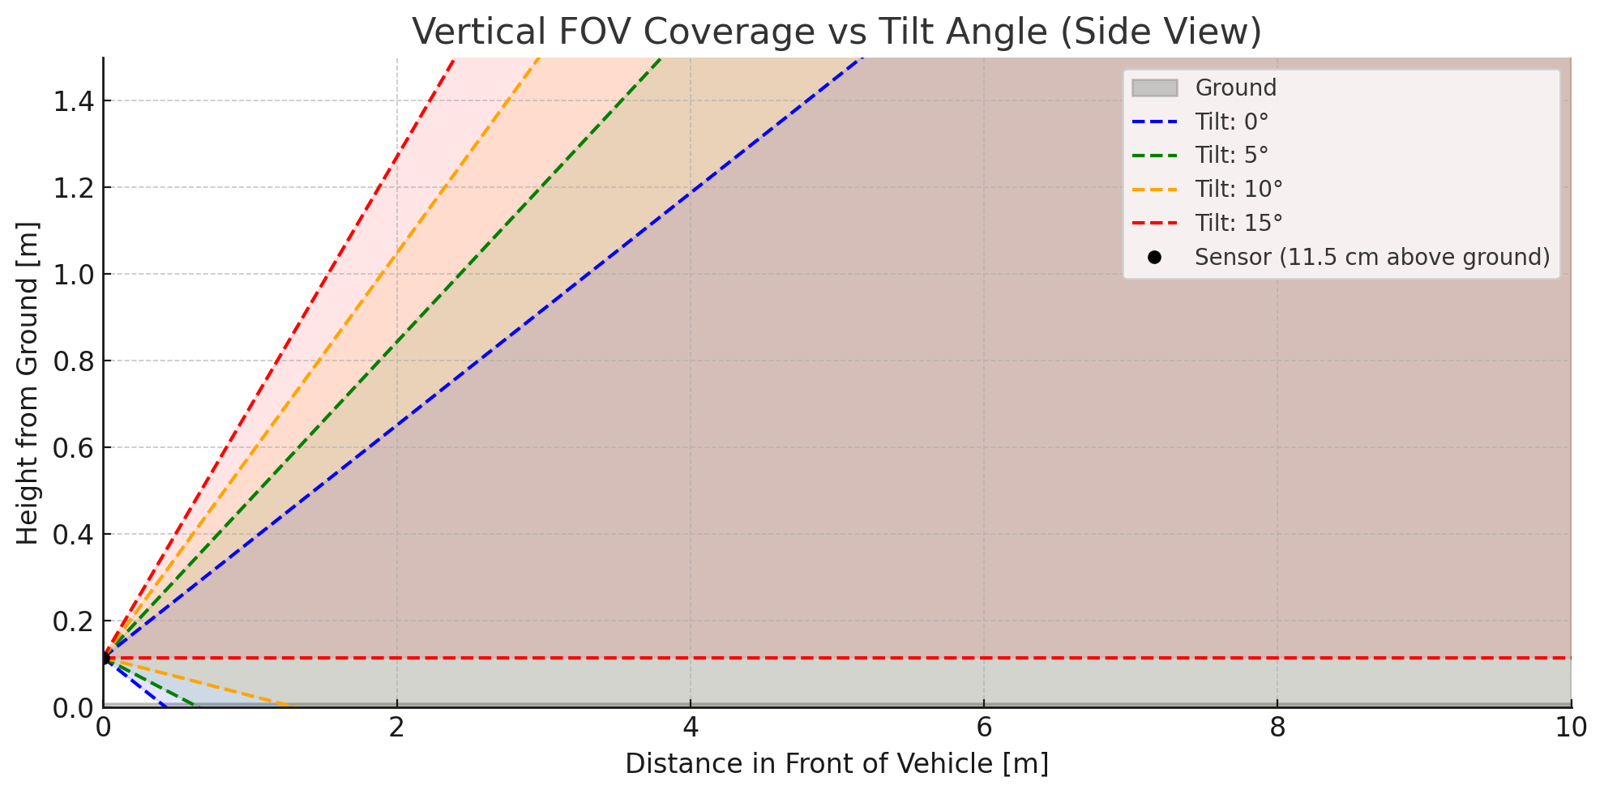
\includegraphics[width=0.8\linewidth]{images/TiltSensor.png}
    \caption{Simulated pitch compensation from $0^\circ$ to $15^\circ$ upward tilt.}
    \label{fig:x_axis_rotation}
\end{figure}

The upward tilt of $15^\circ$ was introduced to minimize clutter from the ground plane.  
With the sensor's vertical FOV of approximately $30^\circ$, this configuration reduced ground clutter while maintaining sufficient detection of obstacles at the intended height range.  
Both the yaw and pitch choices were tested through simulation and validated in real-world mounting experiments (Figures~\ref{fig:z_axis_rotation}, \ref{fig:vehicleRadarYawRotation}, \ref{fig:x_axis_rotation}, \ref{fig:vehicleYawTilt}).

\begin{figure}[!htbp]
    \centering
    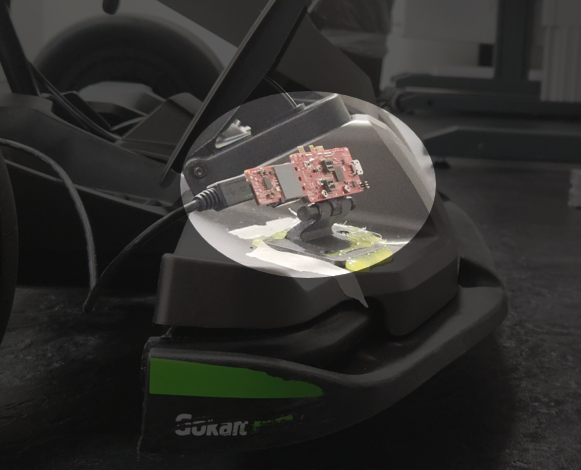
\includegraphics[width=0.8\linewidth]{images/vehicleRadarTiltRotation.png}
    \caption{Real-world implementation of radar tilt ($15^\circ$ upward).}
    \label{fig:vehicleYawTilt}
\end{figure}

\subsubsection{X-Axis Offset Compensation}
After rotation, each sensor's point cloud was translated along the X-axis to align with the vehicle's center:
\begin{itemize}
    \item Radar A: $x \leftarrow x - 0.32$ meters
    \item Radar B: $x \leftarrow x - 0.28$ meters
\end{itemize}

This translation ensured both sensors were aligned in a common vehicle-centric frame.

A yaw rotation \( R_{\text{yaw}} \) was first implemented, followed by a pitch correction \( R_{\text{pitch}} \), and finally a translation vector \( \vec{t} \) was applied to account for the physical position of the sensors with respect to the vehicle's coordinate origin.

\subsubsection{Summary of Extrinsics}
\begin{itemize}
    \item \textbf{Left radar:} yaw $+30^\circ$, pitch $-15^\circ$, translation $(-0.32, 0, 0)$.
    \item \textbf{Right radar:} yaw $-30^\circ$, pitch $-15^\circ$, translation $(-0.28, 0, 0)$.
\end{itemize}

This extrinsic calibration ensures that dual-radar data is expressed in a coherent vehicle-centric frame, which is critical for downstream modules such as clustering, odometry, and obstacle tracking.

\newpage
\subsection{Radar Merge}  
\indent Once each radar's detections were transformed into the common vehicle frame, the two datasets were merged into a single unified point cloud per frame.  
This step ensured that detections from both radars contributed consistently to the pipeline.  

This fusion improves both density and coverage, particularly in regions where the individual radar fields of view overlap.  
It also reduces ambiguity during clustering, since targets detected by both sensors reinforce one another once aligned.  

The effect of merging is visualized in Fig.~\ref{fig:radar_merge}, where the independent point clouds (top) are combined into a single dataset (bottom).  

\begin{figure}[!htbp]
    \centering
    \begin{subfigure}[t]{0.8\linewidth}
        \centering
        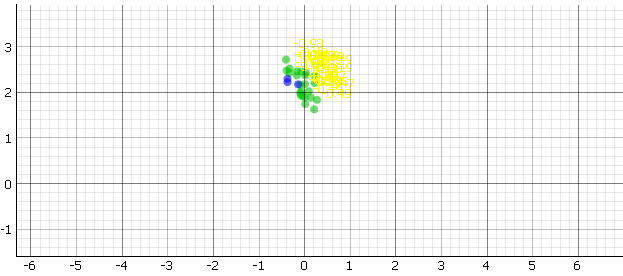
\includegraphics[width=\linewidth]{images/AFTERdualSensorCalib_2mts.png}
        \caption{Independent point clouds before merging.}
    \end{subfigure}
    \vfill
    \begin{subfigure}[t]{0.8\linewidth}
        \centering
        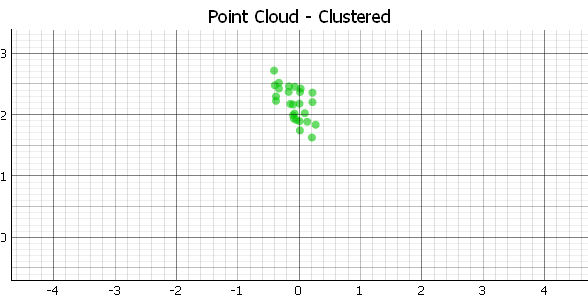
\includegraphics[width=\linewidth]{images/AFTERdualSensorCalibCluster_2mts.png}
        \caption{Unified point cloud after merging.}
    \end{subfigure}
    \caption{Radar merge process: alignment of calibrated detections into a single dataset. (a) Radar A = blue, Radar B = green. (b) Merged point cloud.}
    \label{fig:radar_merge}
\end{figure}


\section{Summary and Outlook}

% Summary and leasons learned
In this project, an object detection system for a consumer-grade electric go-kart was implemented by using a mmWave radar sensor.
The system successfully meets its primary objectives by accurately detecting obstacles through a custom point-cloud analysis algorithm.
Although the current implementation is limited to stationary objects, it establishes a strong foundation for future development.
All necessary components, including a modular processing pipeline and a hardware interface for safely manipulating the go-kart's brake signal, were developed.
\par
The pipeline's modular architecture proved to support a dynamic developing process, which turned out to be necessary when working with point clouds from radar sensors and an electric go-kart that was not intended to be modified by the end-user.
It also enables further development by expanding, exchanging or modifying processing stages.
During the development, two stages turned out to be extraordinary helpful when it comes to mitigating the influences of the potentially heavily fluctuating point cloud data.
The frame aggregator in combination with running the radar sensor at a high frame rate successfully tackled the problem of data sparsity that sometimes occurred in the test scenario environment.
This was caused by the scenario's "clean" setup without a huge number of targets.
The two-stage clustering approach using the DBSCAN algorithm proved to be able to reliably filter out outliers caused by clutter or noise and was able to provide the brake controller with stable information on stationary objects.
\par
In addition to those two stages, the usage of multiple filtering stages of static and dynamic behavior proved to support the reliability of the whole system.
Static filtering stages early in the pipeline are able to filter out irrelevant points or those with a low level of confidence by using their spatial coordinates and $SNR$ information.
This reduces the required processing time of the later stages by condensing the mass of data to the relevant points.
The dynamic filtering stage allows a reliable differentiation between points that are caused by stationary and moving targets by leveraging the information of the radar-only self-speed estimation.
The approach of using a distance that is linear to the vehicle's velocity to decide whether an emergency braking event should be triggered, and outputting a binary signal, turned out to be sufficient, as the balance board's internal controller prevents the wheels from locking.
\par\bigskip
As with any project, there is always room for improvement, and this work is no exception.
Although the current implementation meets the initial goals and requirements, the algorithm can still be refined.
The project is currently implemented in a threaded solution using Python, which is a result of the dynamic development process where a lot of different techniques and approaches where implemented, tested and sometimes discarded.
Switching from C++, which was used initially used for development, to Python allowed for a quicker development with simpler possibilities of visualization, but also caused a noticeable lack of performance.
This lack of performance showed up in the last stages of development, during testing, and created a delay in the response when tested in an autonomous environment, meaning that when the implementation was not powered by a sufficient power supply, the implemented system showed certain delays in the response when an object was detected in the area for activation of the brake.
It is assumed that the delay originates from Python's heavyweight interpreter and should vanish after porting the system's implementation back to C++.
As for this reason, the decision of not fully merging the existing system into the test vehicle at this stage of the development was made, as it did not provided a fully safe environment for testing.
The validation was done with a LED to indicate the activation of the emergency brake.
An improvement or next step would be to migrate the system back to C++, where the threaded implementation would provide a better response time for each running task.
Further improvements can also be made by incorporating occupancy grids through a Bayesian filter to enhance object detection, allowing the system to go beyond stationary targets.
By improving the system's object detection capabilities to cover moving targets, it would also be possible to estimate their direction of movement, which could significantly improve the driving assistance algorithm and contribute to accident prevention through a more precise analysis.
\par\bigskip
The present status of this project is available in the following GitHub repository: \href{https://github.com/LF-RoGu/Radar-mmWave}{Radar-mmWave on GitHub}.
%\section{WIP - Storing TikZ graphics}

\begin{figure}[!htbp]
    \centering
    \resizebox{0.48\textwidth}{!}{
        \begin{tikzpicture}
            % Block styles
            \tikzstyle{block} = [rectangle, draw, text width=4.5em, text centered, minimum width=6em, minimum height=4em]
            \tikzstyle{block_dashed} = [rectangle, draw, text width=2em, text centered, minimum width=4em, minimum height=4em, dashed]
            % Input and output
            \node[block, right=of antenna, minimum width=4em, minimum height=4em] (frames) {Frames};
            \node[block, right=of frames] (frame_aggr) {Frame\\Aggregator};
            \node[block, right=of frame_aggr] (coord_filter) {Filter\\$x,y,z$\\$\phi,SNR$};
            \node[block, right=of coord_filter] (self_speed_estim) {Self-speed Estimator};
            \node[block, right=of self_speed_estim] (self_speed_kalman) {Kalman Filter};
            \node[block, below=of self_speed_estim] (ve_speed_calc) {Calculation\\of $v_{e}$};
            \node[block, right=of ve_speed_calc] (ve_filter) {Filter\\$v_{e}$ vs. self-speed};
            \node[block, right=of ve_filter] (clustering) {Clustering};
            % Connections
            \draw[->] (frames) -- (frame_aggr); % Connection from antenna to RF amplifier
            \draw[->] (frame_aggr) -- (coord_filter);
            \draw[->] (coord_filter) -- (self_speed_estim);
            \draw[->] (coord_filter.south) |- (ve_speed_calc.west);
            \draw[->] (self_speed_estim) -- (self_speed_kalman);
            \draw[->] (self_speed_kalman) -- (ve_filter);
            \draw[->] (ve_speed_calc) -- (ve_filter);
            \draw[->] (ve_filter) -- (clustering);
        \end{tikzpicture}
    }
    \caption{Block diagram of the pipeline}
    \label{fig:block_diag_pipeline}
\end{figure}

\begin{figure}[!htbp]
    \centering
    \resizebox{0.48\textwidth}{!}{
        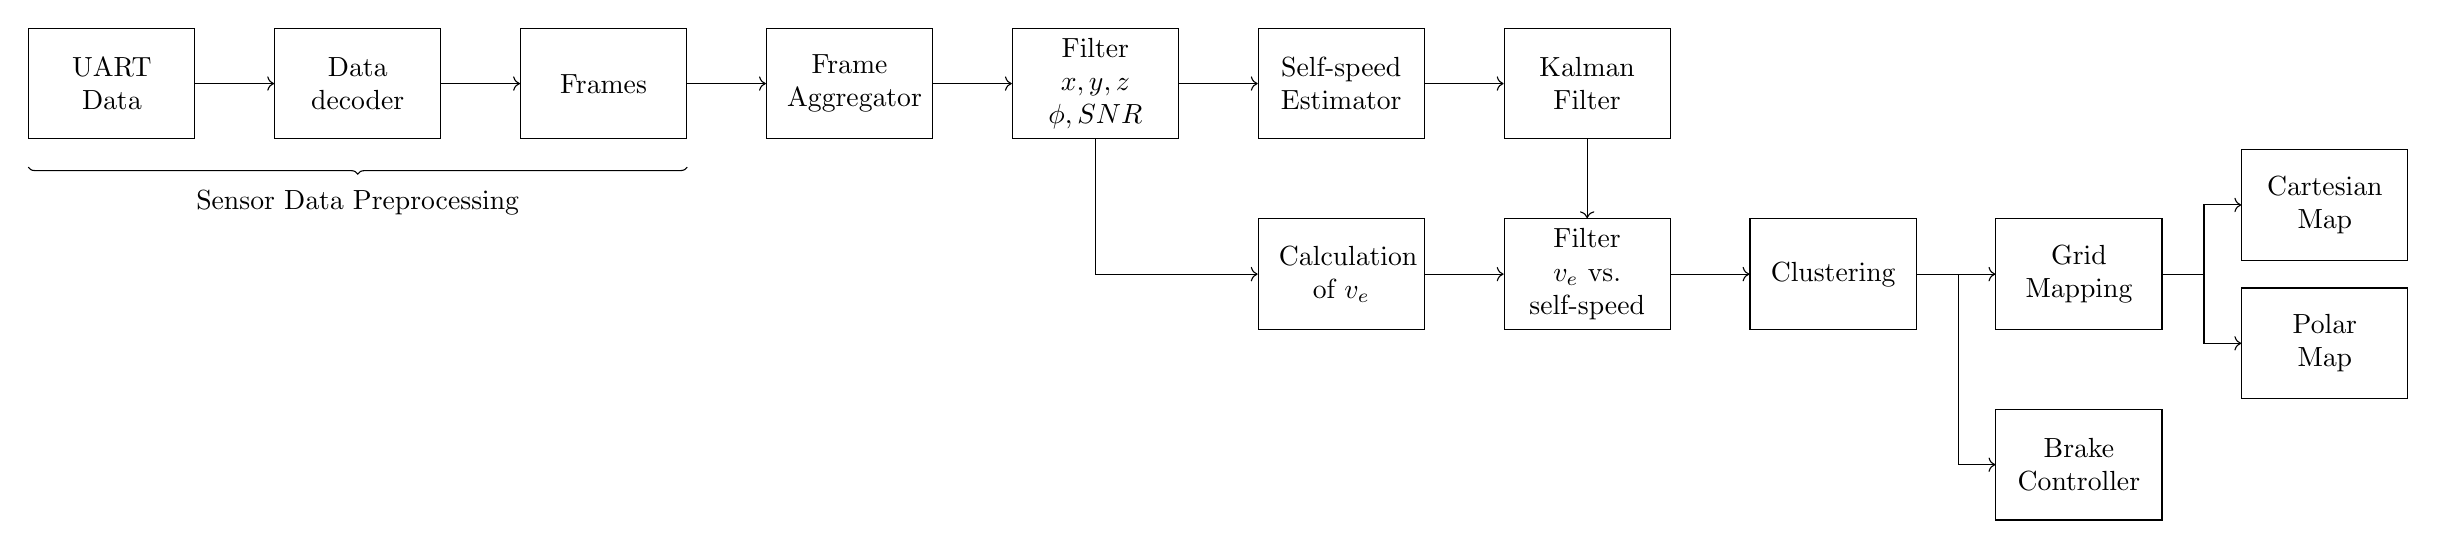
\begin{tikzpicture}
            % Block styles
            \tikzstyle{block} = [rectangle, draw, text width=4.5em, text centered, minimum width=6em, minimum height=4em]
            \tikzstyle{block_dashed} = [rectangle, draw, text width=2em, text centered, minimum width=4em, minimum height=4em, dashed]
            % Input and output
            \node[block] (uart) {UART\\Data};
            \node[block, right=of uart] (decoder) {Data decoder};
            \node[block, right=of decoder] (frames) {Frames};
            \node[block, right=of frames] (frame_aggr) {Frame\\Aggregator};
            \node[block, right=of frame_aggr] (coord_filter) {Filter\\$x,y,z$\\$\phi,SNR$};
            \node[block, right=of coord_filter] (self_speed_estim) {Self-speed Estimator};
            \node[block, right=of self_speed_estim] (self_speed_kalman) {Kalman Filter};
            \node[block, below=of self_speed_estim] (ve_speed_calc) {Calculation\\of $v_{e}$};
            \node[block, right=of ve_speed_calc] (ve_filter) {Filter\\$v_{e}$ vs. self-speed};
            \node[block, right=of ve_filter] (clustering) {Clustering};
            \node[block, right=of clustering] (grid_mapping) {Grid Mapping};
            \node[block, right=of grid_mapping.east, yshift=2.5em] (grid_cartesian) {Cartesian\\Map};
            \node[block, right=of grid_mapping.east, yshift=-2.5em] (grid_polar) {Polar\\Map};
            \node[block, below=of grid_mapping] (brake) {Brake\\Controller};
            % Connections
            \draw[->] (uart) -- (decoder);
            \draw[->] (decoder) -- (frames);
            \draw[->] (frames) -- (frame_aggr); % Connection from antenna to RF amplifier
            \draw[->] (frame_aggr) -- (coord_filter);
            \draw[->] (coord_filter) -- (self_speed_estim);
            \draw[->] (coord_filter.south) |- (ve_speed_calc.west);
            \draw[->] (self_speed_estim) -- (self_speed_kalman);
            \draw[->] (self_speed_kalman) -- (ve_filter);
            \draw[->] (ve_speed_calc) -- (ve_filter);
            \draw[->] (ve_filter) -- (clustering);

            \draw[-] (clustering.east) --++(1.5em, 0) coordinate (arrw_clustering);
            \draw[->] (arrw_clustering) -- (grid_mapping);
             \draw[->] (arrw_clustering) |- (brake);

            \draw[-] (grid_mapping.east) --++(1.5em, 0) coordinate (arrw_mapping_grids);
            \draw[->] (arrw_mapping_grids) |- (grid_cartesian.west);
            \draw[->] (arrw_mapping_grids) |- (grid_polar);

            \draw [decorate, decoration = {brace, mirror, raise=10pt}] (uart.south west) --  (frames.south east) node[pos=0.5,below=15pt,black]{Sensor Data Preprocessing};
        \end{tikzpicture}
    }
    \caption{Block diagram of the pipeline}
    \label{fig:block_diag_pipeline}
\end{figure}


\begin{figure}[!htbp]
    \centering
    \resizebox{0.48\textwidth}{!}{
        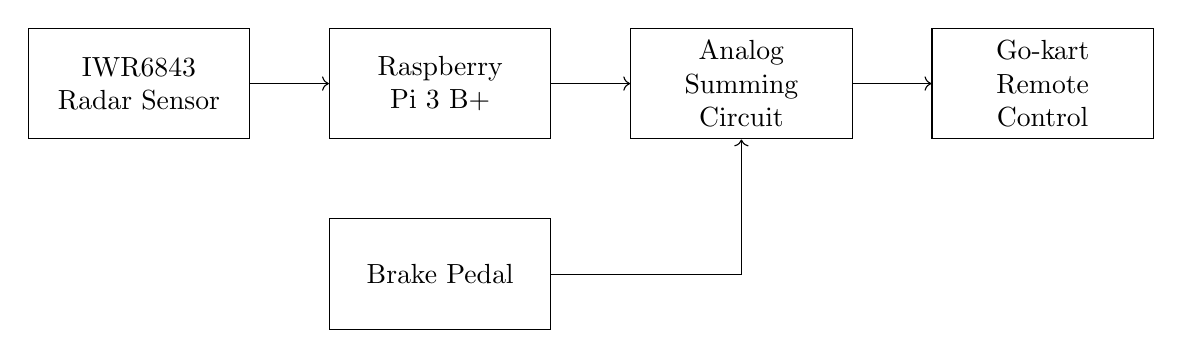
\begin{tikzpicture}
            % Block styles
            \tikzstyle{block} = [rectangle, draw, text width=6.5em, text centered, minimum width=8em, minimum height=4em]
            \tikzstyle{block_dashed} = [rectangle, draw, text width=2em, text centered, minimum width=4em, minimum height=4em, dashed]
            % Input and output
            \node[block] (radar) {IWR6843\\Radar Sensor};
            \node[block, right=of radar] (rpi) {Raspberry\\Pi 3 B+};
            \node[block, right=of rpi] (analog_summ) {Analog Summing\\Circuit};
            \node[block, below=of rpi] (brake_pedal) {Brake Pedal};
            \node[block, right=of analog_summ] (remote) {Go-kart\\Remote Control};
            % Connections
            \draw[->] (radar) -- (rpi);
            \draw[->] (rpi) -- (analog_summ);
            \draw[->] (brake_pedal) -| (analog_summ);
            \draw[->] (analog_summ) -- (remote);
        \end{tikzpicture}
    }
    \caption{Block diagram of the pipeline}
    \label{fig:block_diag_pipeline}
\end{figure}
\newpage

\begin{thebibliography}{00}

\bibitem{ninebot_product_page} Segway Inc., ``Ninebot Go-kart PRO product page'', 2025, Webpage. [Online]. Available: \url{https://de-de.segway.com/products/ninebot-gokart-pro}

\bibitem{iwr_awr_diff} Texas Instruments, ``IWR1642: difference between AWR and IWR parts'', 2025, Webpage. [Online]. Available: \url{https://e2e.ti.com/support/sensors-group/sensors/f/sensors-forum/742730/iwr1642-difference-between-awr-and-iwr-parts}

\bibitem{dev_board_page} Texas Instruments, ``IWR6843AOPEVM product page'', 2025, Webpage. [Online]. Available: \url{https://www.ti.com/tool/IWR6843AOPEVM}

\bibitem{mmwave_demo_doc} Texas Instruments, ``User's Guide mmWave Demo Visualizer,'' 2020, Online Document. [Online]. Available: \url{https://www.ti.com/lit/ug/swru529c/swru529c.pdf?ts=1742817596204}.

\bibitem{understanding_uart} Texas Instruments, ``Understanding UART Data Output Format'', 2025, Webpage. [Online]. Available: \url{https://dev.ti.com/tirex/content/radar_toolbox_2_20_00_05/docs/software_guides/Understanding_UART_Data_Output_Format.html}

\bibitem{mmwave_demo_output} Texas Instruments, ``mmWave Sensing Estimator'', 2025, Webpage. [Online]. Available: \url{https://dev.ti.com/gallery/view/mmwave/mmWaveSensingEstimator/ver/2.5.1/}


\bibitem{ninebot_protocol_github} ub4raf, ``Ninebot-PROTOCOL'', 2025, GitHub Repository. [Online]. Available: \url{https://github.com/ub4raf/Ninebot-PROTOCOL}

\bibitem{ninebot_protocol_scooterhacking} -, ``Ninebot ES Communicaton Protocol'', 2019, Webpage. [Online]. Available: \url{https://cloud.scooterhacking.org/release/nbdoc.pdf}

\bibitem{numpy_polyfit} -, ``numpy.polyfit documentation'', 2025, Webpage. [Online]. Available: \url{https://numpy.org/doc/stable/reference/generated/numpy.polyfit.html}

\bibitem{OccupancyGrid_Mapping_Automotive} Ç. Önen, A. Pandharipande, G. Joseph, and N. J. Myers, ``Occupancy Grid Mapping for Automotive Driving Exploiting Clustered Sparsity,'' \textit{IEEE Sensors Journal}, vol. 24, no. 7, pp. 9240-9250, 2024. [Online]. Available: \url{https://doi.org/10.1109/JSEN.2023.3342463}.

\bibitem{Odometry_radar_only}
D. Casado Herraez, M. Zeller, L. Chang, I. Vizzo, M. Heidingsfeld, and C. Stachniss, 
``Radar-Only Odometry and Mapping for Autonomous Vehicles,'' 
\textit{arXiv preprint}, 2023. [Online]. Available: \url{https://arxiv.org/abs/2305.12409}

\bibitem{EgoMotion_DopplerRadar}
S. R. Bhatt, B. S. Nadiger, R. Parthasarathy, and H. M. Shetty, 
``Instantaneous Ego-motion Estimation Using Doppler Radar,'' 
\textit{IEEE Sensors Letters}, vol. 7, no. 5, pp. 1–4, 2023. [Online]. Available: \url{https://doi.org/10.1109/LSENS.2023.3244030}

\bibitem{Multimodal_Offroad}
C. E. Beal, T. Williams, J. Pauli, M. Mukadam, and B. Boots, 
``Robust Off-Road Autonomy Using Multimodal Sensor Fusion,'' 
in \textit{Proc. of the Conference on Robot Learning (CoRL)}, 2023. [Online]. Available: \url{https://openreview.net/forum?id=kmiZqSgoAt}

\bibitem{HighSpeed_Estimation}
B. Sundaralingam, C. E. Beal, and B. Boots, 
``Robust High-Speed State Estimation for Off-Road Autonomous Vehicles,'' 
in \textit{Proc. of Robotics: Science and Systems (RSS)}, 2023. [Online]. Available: \url{https://openreview.net/forum?id=3JpFLY3ihix}


\bibitem{geeksforgeeks_dbscan}
GeeksforGeeks, 
\emph{DBSCAN Clustering in ML | Density Based Clustering}, 
2023. [Online]. Available: \url{https://www.geeksforgeeks.org/dbscan-clustering-in-ml-density-based-clustering/}. [Accessed: 19-Mar-2025].

\bibitem{mathworks_kalman}
MathWorks,
\textit{Understanding Kalman Filters, Part 3: Optimal State Estimator},
2017. Available at: \url{https://la.mathworks.com/videos/understanding-kalman-filters-part-3-optimal-state-estimator--1490710645421.html} (Accessed: March 23, 2025).

\bibitem{ti_radar_toolbox}
Texas Instruments, 
\textit{Radar Toolbox – mmWave Sensor Configuration and Demos}, 
2024. Available at: \url{https://dev.ti.com/tirex/explore/node?node=A__ADnbI7zK9bSRgZqeAxprvQ__radar_toolbox__1AslXXD__2.20.00.05} (Accessed: March 23, 2025).




\end{thebibliography}


\end{document}

\begin{comment}
    [26/09/2025]
    [Guide Outline — Pre-thesis Structure]

    Abstract  
    - High-level summary: problem → method → key results → significance.  

    Introduction  
    - Background (odometry, current methods).  
    - Motivation (why radar odometry, why this project).  
        - General objective: main project goal.
    - Research gap (what existing methods lack).  
    - Contribution statement (what you did).
        - Without going into technical details.
        - Without doing into depth.

    SYSTEM DESIGN AND METHODOLOGY
        Research design
            - Explain the conceptual and mathematical framework.
            - Specific objectives: concrete steps
                - Design mounts (conceptual justification, not CAD details).
                - Configure chirps (parameters, mathematical rationale).
                - Implement filtering pipeline (mathematical description).
                    - Show pipeline diagram here (block diagram).

        System Hardware
            - Sensors (radar, IMU, webcam).
            - Mechanical integration (3D printed mounts, placement).
            - Sensor configuration
                - Radar setup.
                    - Sensor configuration.
                    - Sensor transformations.
                    - Chirp configuration.
                - IMU setup.
            * Keep at a descriptive/theoretical level (role of each hardware element in methodology). 

        Methodology (Pipeline)
            - Present the pipeline as the method.
            - Each subsection = one module (Transformations, Frame Aggregation, RANSAC, Clustering, ICP).
            - For each: explain mathematical approach, algorithm logic, expected effect.
            - Show diagrams (block flowcharts, data transformations).
            - End with summary of expected advantages of this design.

    Implementation & Experimental Setup (Showcasing your work)
        - Describe actual implementation process (code, synchronization, data collection).
        - Explain experimental platform (Ninebot test vehicle, dual radars, IMU, lab environment).
        - Show photos/screenshots (sensor mounts, test tracks, visualizations).
        - Here we describe *how it was realized in practice*, not the math.  

    Results & Discussion
    - Initial results (trajectory plots, ego-speed estimation, cluster visualization).  
    - Comparison with previous work (paper approach, wheel encoder, or naive ICP).  
        - Compare with full ICP vs cluster ICP.
    - Discuss successes and limitations.  

    Future Work  
    - Interpret results: where radar odometry shines, where it struggles.  
    - How your design choices (dual radars, chirp config, RANSAC filtering) affected performance.  

    Conclusion 
    - Wrap up contributions.  
    - Highlight possible extensions (sensor fusion, better clustering, real-world driving).  

    Bibliography  
\end{comment}
